\documentclass[dvipsnames]{beamer}
\usepackage{xcolor}
\usepackage{graphicx}
\usepackage{listings}

\usetheme{Madrid}
\usecolortheme{beaver}
\date[26 September 2025]{}

\title[SUMO, Curriculums and MARL]{Unconventional reinforcement learning on traffic lights with SUMO}
\subtitle{Master Degree in Computer Science}
% \author{Refolli~F.~865955}
\author[R.F. 865955]{Francesco~Refolli\\[10mm]{\small Supervisor: Prof. Giuseppe Vizzari}}
\logo{
\includegraphics[height=2.5cm]{logo_unimib.pdf}}

\newcommand{\putimage}[2] {
  \begin{figure}[H]
    \centering
    \includegraphics[width=#2\linewidth]{#1}
	\end{figure}
}

\newcommand{\putimagecouple}[4] {
  \begin{figure}[!htb]
    \centering
    \begin{minipage}{0.45\linewidth}
      \centering
      \includegraphics[width=\linewidth]{#1}
      \caption{#2}
    \end{minipage}
    \hspace{0.25cm}
    \begin{minipage}{0.45\linewidth}
      \centering
      \includegraphics[width=\linewidth]{#3}
      \caption{#4}
    \end{minipage}
  \end{figure}
}

\begin{document}

\frame{\titlepage}

\setbeamertemplate{logo}{}

\begin{frame}
\frametitle{Outline}
\tableofcontents
\end{frame}

\section{Introduction}
\begin{frame}
\centering
\Huge
Introduction
\end{frame}

\begin{frame}
  \frametitle{Problem statement}

  This thesis dealt with the Traffic Light Control problem (TCL) applying uncommon reinforcement learning techniques.
  In particular, the following research objective were pursued in the performed experiments:

  \begin{itemize}
    \item \textcolor{SeaGreen}{Evaluating the effectiveness of Curriculum Learning}
    \item \textcolor{SeaGreen}{Evaluating the effectiveness of Multi Agent Learning}
    \item \textcolor{CadetBlue}{Evaluating the effectiveness of Self-Adaptive agents}
    \item \textcolor{CadetBlue}{Comparing observation/reward functions}
    \item \textcolor{CadetBlue}{Comparing tabular and deep learning models}
    \item \textcolor{CadetBlue}{Comparing Reinforcement Learning with existing solutions}
    \item \textcolor{CadetBlue}{Evaluating the role of hyperparameters}
  \end{itemize}
\end{frame}

\begin{frame}
  \begin{columns}
    \begin{column}{0.4\textwidth}
      \begin{figure}
        \centering
        
\includegraphics[width=1.0\textwidth]{figures/sumo-logo.png}
      \end{figure}
      \begin{itemize}
        \item Free and Open Source microscopic traffic simulator
        \item Developed at German Aerospace Center (DLR)
        \item Multimodal: cars, trams, bikes, pedestrians ...
        \item Highly customizable
      \end{itemize}
    \end{column}
    \begin{column}{0.6\textwidth}
      \begin{figure}
        \centering
        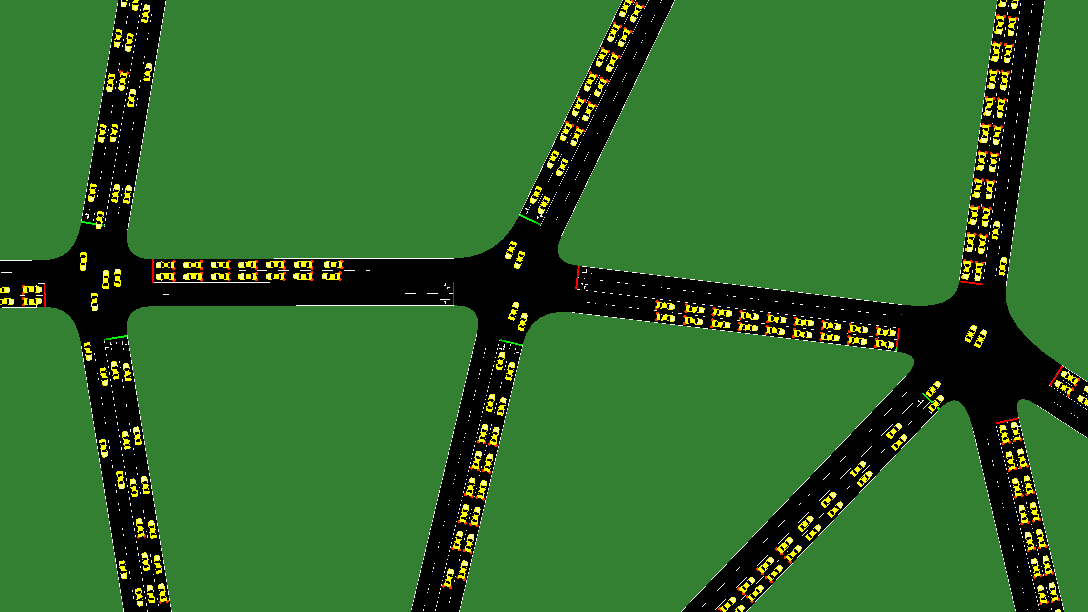
\includegraphics[width=1.0\textwidth]{figures/sumo-example.png}
      \end{figure}
      \begin{figure}
        \centering
        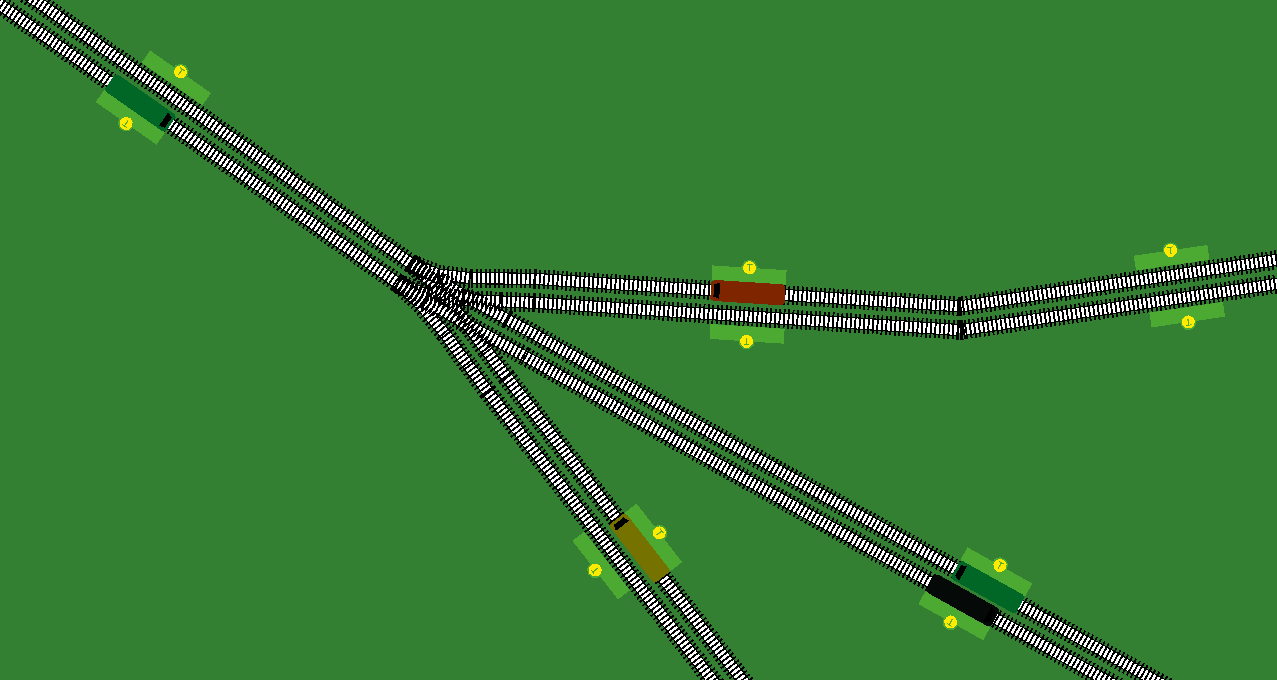
\includegraphics[width=1.0\textwidth]{figures/sumo-example2.png}
      \end{figure}
    \end{column}
  \end{columns}
\end{frame}

\begin{frame}
\frametitle{SUMO-RF: SUMO + Reinforcement Learning}
  A FOSS framework for Reinforcement Learning with SUMO developed as fork of \textit{LucasAlegre/sumo-rl} with a focus on modularity, flexibility and Multi Agent Learning.
  It also contains several utilities for format conversions, metrics analysis and plot, schematic-based demand generation and more.
  \begin{figure}
    \centering
    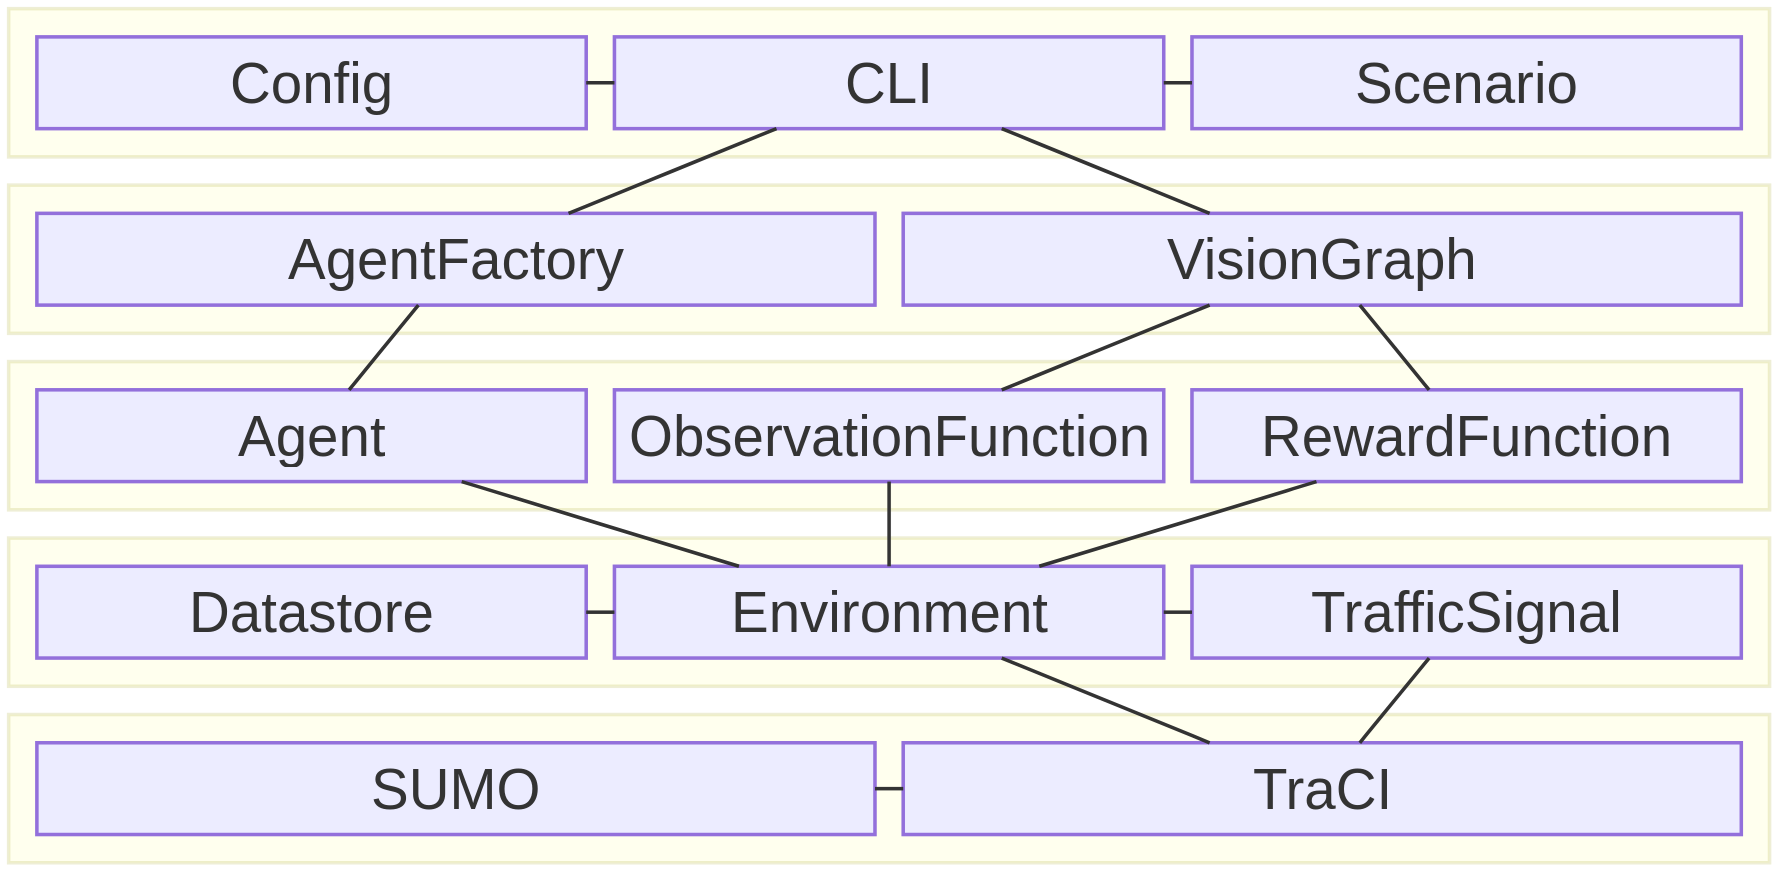
\includegraphics[width=0.8\textwidth]{figures/sumo-rf-architecture.png}
  \end{figure}
\end{frame}

\begin{frame}
\frametitle{The scenario}
  \begin{figure}
    \centering
    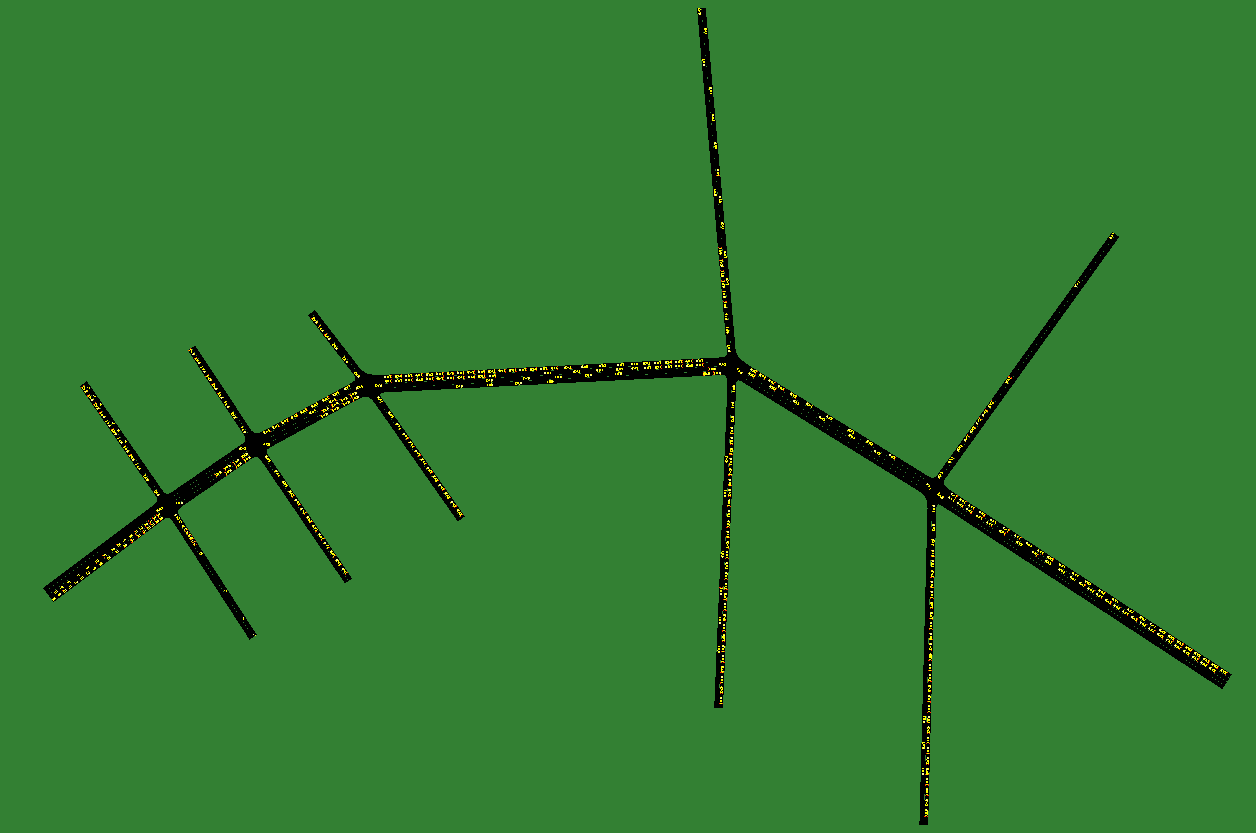
\includegraphics[width=1.0\textwidth]{figures/sumo-bassini.png}
  \end{figure}
\end{frame}

\begin{frame}
\frametitle{The Agent Model}
  \begin{columns}
    \begin{column}{0.6\textwidth}
    {\small
    \begin{itemize}
      \item Each agent can control one intersection and at each step (every 5 seconds) it can choose the next phase of the intersection.
      \item Every action is automatically enforced by TrafficSignal with also an intermediate yellow phase.
      \item It receives an observation of the current condition and a reward proportional to the goodness of its behaviour.
      \item If the agent is "smart", it uses the collected data to improve itself!
    \end{itemize}}
    \end{column}
    \begin{column}{0.4\textwidth}
      \begin{figure}
        \centering
        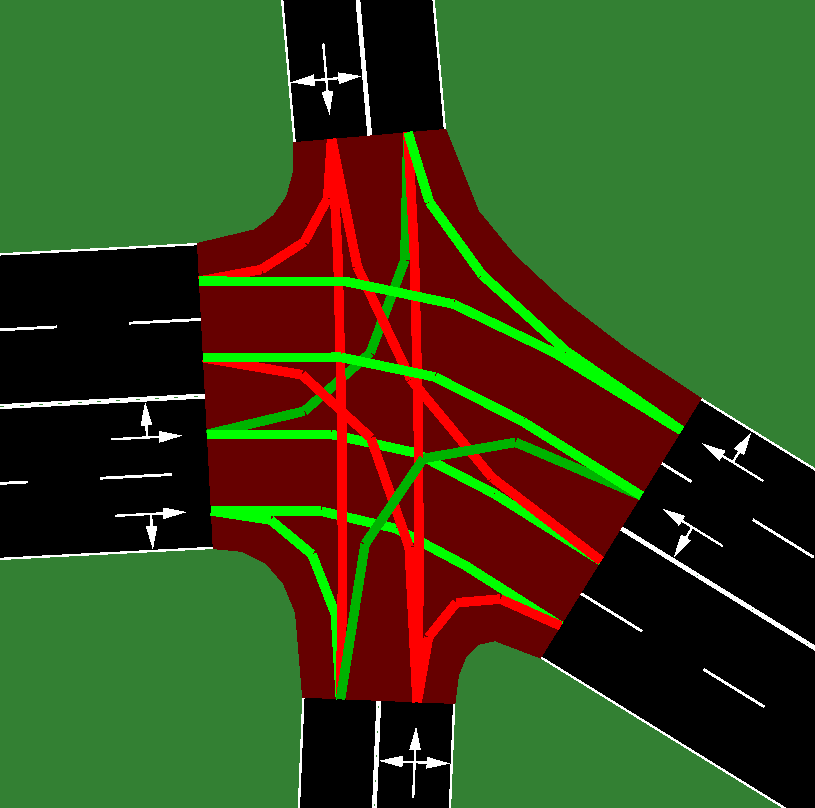
\includegraphics[width=1.0\textwidth]{figures/sumo-rf-agent.png}
      \end{figure}
    \end{column}
  \end{columns}
\end{frame}

\begin{frame}
\frametitle{The Global State}
  \begin{figure}
    \centering
    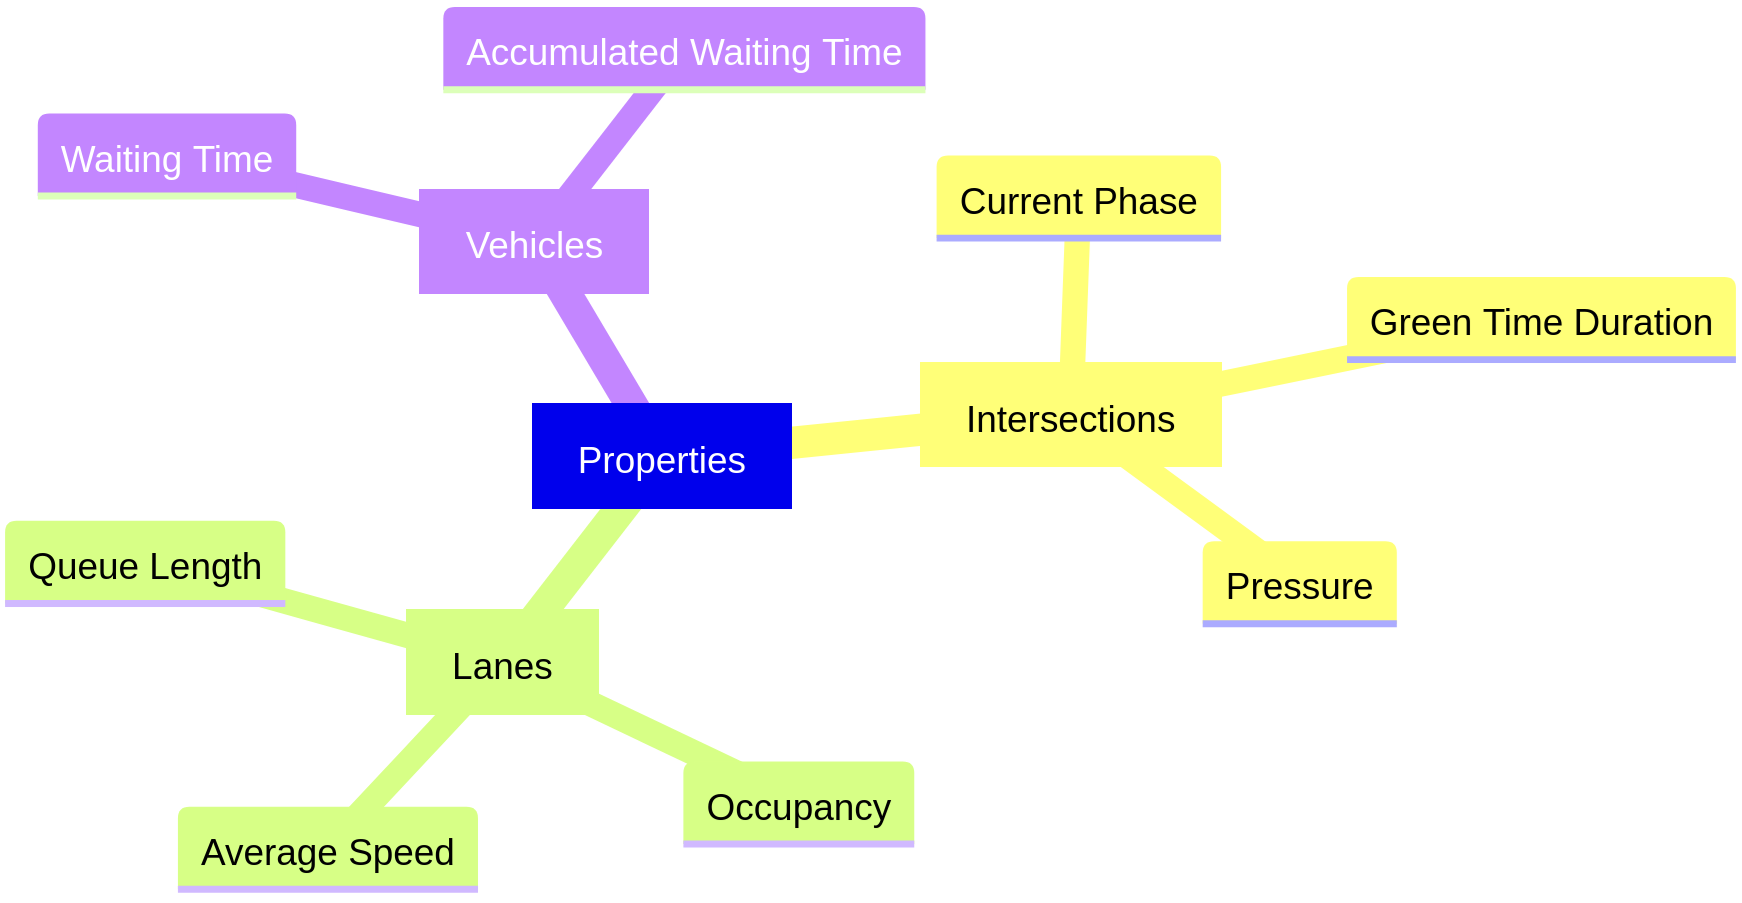
\includegraphics[width=1.0\textwidth]{figures/sumo-rf-properties.png}
  \end{figure}
\end{frame}

\begin{frame}
\frametitle{Observing and Rewarding}
  \begin{columns}
  \begin{column}{0.4\textwidth}
    \begin{figure}
      \centering
      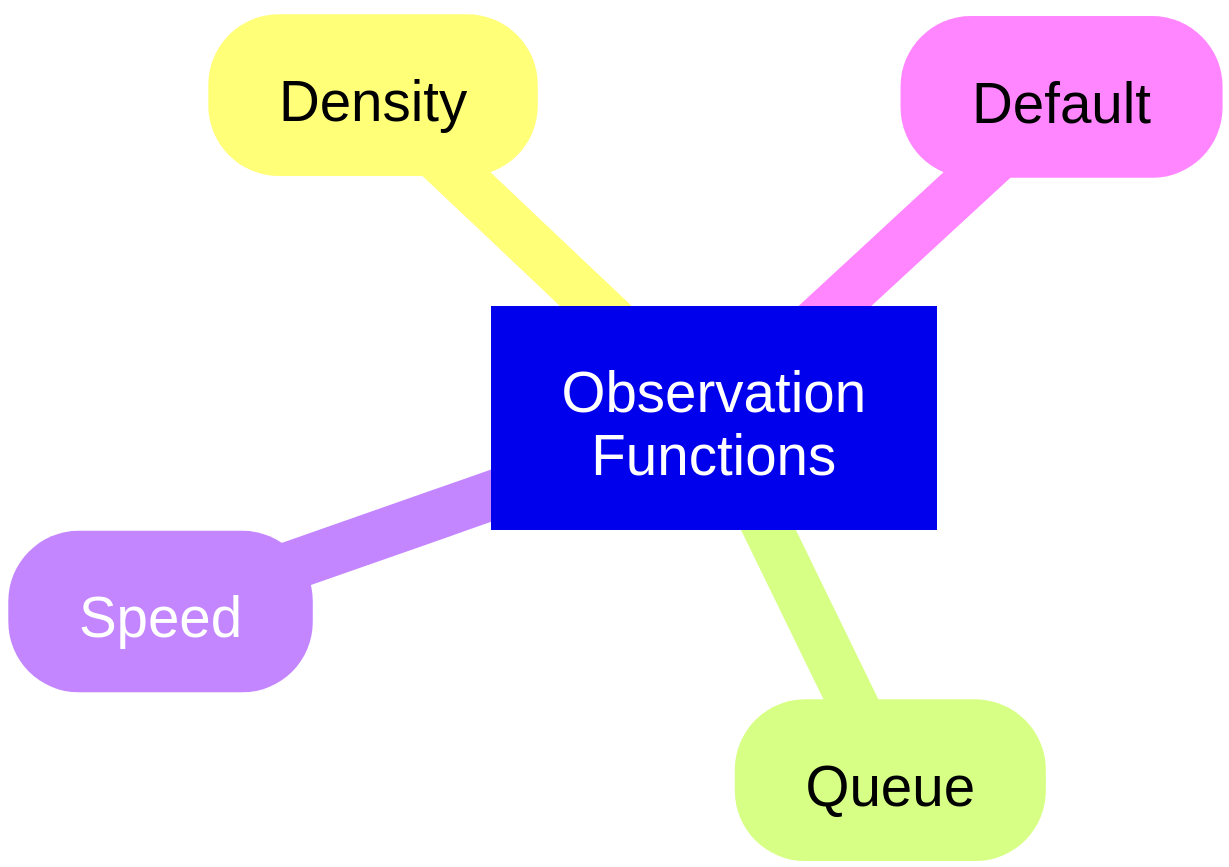
\includegraphics[width=1.0\textwidth]{figures/sumo-rf-observations.png}
    \end{figure}
  \end{column}
  \begin{column}{0.6\textwidth}
    \begin{figure}
      \centering
      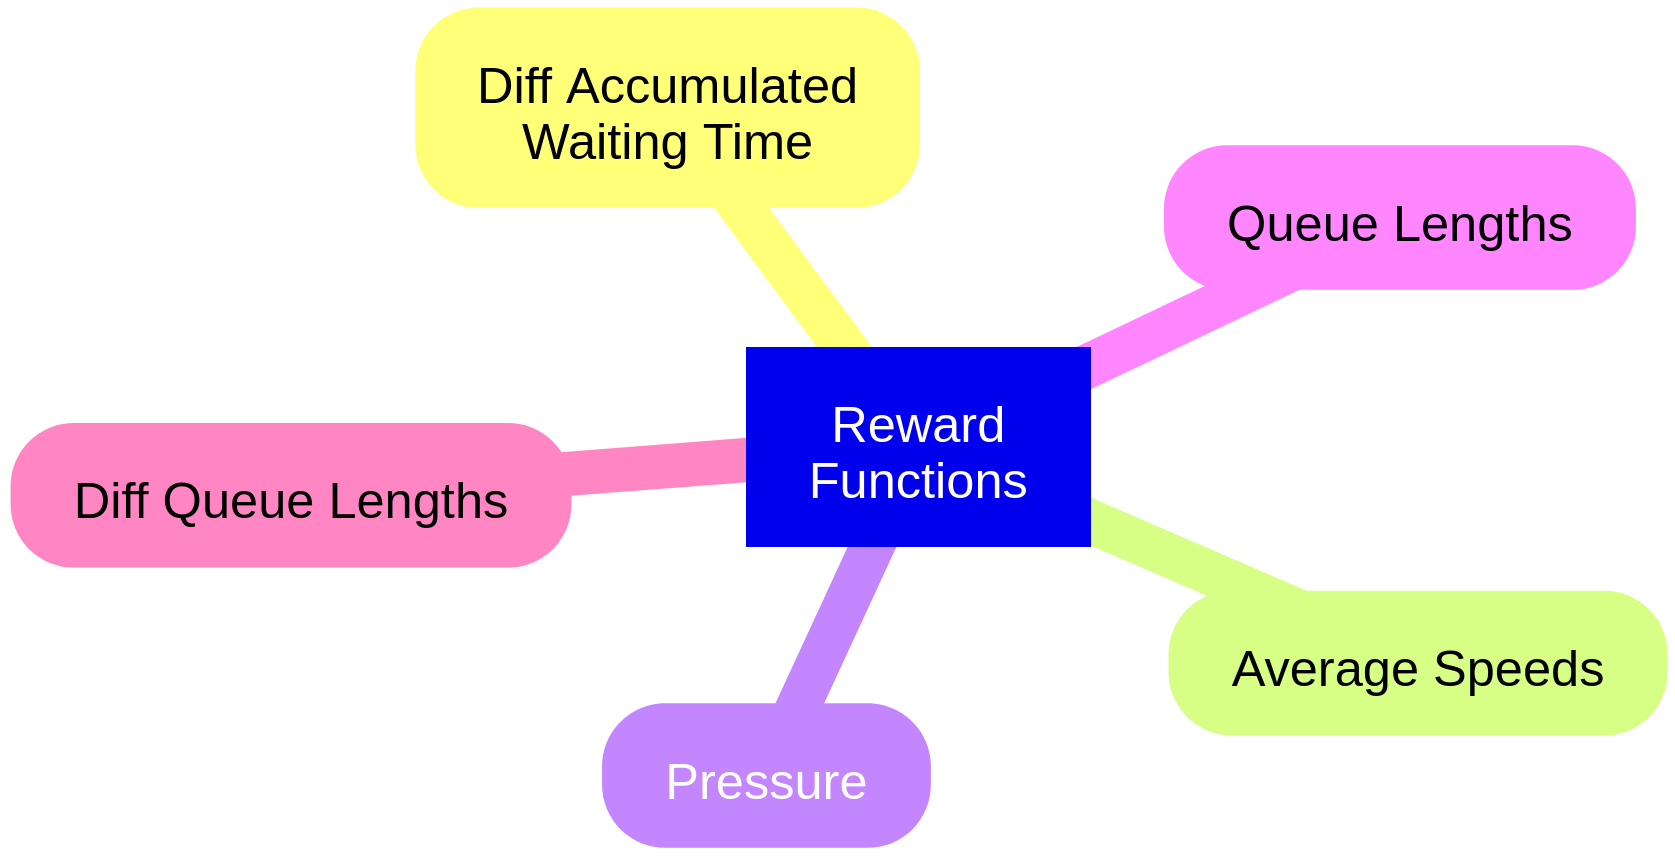
\includegraphics[width=1.0\textwidth]{figures/sumo-rf-rewards.png}
    \end{figure}
  \end{column}
\end{columns}
\end{frame}

\section{Curriculum Learning}
\begin{frame}
\centering
\Huge
Curriculum Learning
\end{frame}

\begin{frame}
\frametitle{Experience Engineering}
  \begin{itemize}
    \item Unlike classic RL problems like CartPole, here the configured demand over time of the system is actually a hyperparameter.
    \item In order to train and evaluate the agents a schematic of demand ("dataset") shall be created resembling both daily conditions and abnormal conditions.
    \item Since there are many junctions, many entry/exit points and each flow intensity can vary significantly, the complexity of a scenario is high.
  \end{itemize}
  
  Two approaches:
  \begin{itemize}
    \item \textbf{Monolithic}: systematically train the agents against almost all combinations of subtaks.
    \item \textbf{Curriculum}: train the agents against each subtask in isolation expecting the agents to generalize their knowledge.
  \end{itemize}
  
  %\textcolor{SeaGreen}{
  %\textcolor{SeaGreen}{
  %Bonus:
  %\begin{itemize}
  %  \item \textcolor{SeaGreen}{\textbf{Incremental learning}: train the agents with examples of increasing complexity/intensity.}
  %  \item \textcolor{CadetBlue}{\textbf{Experience replay}: record $({S}_{t-1}, {A}_{t-1}, {S}_{t-1}, {R}_{t-1})$ samples and present them to the agents in random batches.}
  %\end{itemize}
\end{frame}

\begin{frame}
\frametitle{A modular learning framework}
  \begin{figure}
    \centering
    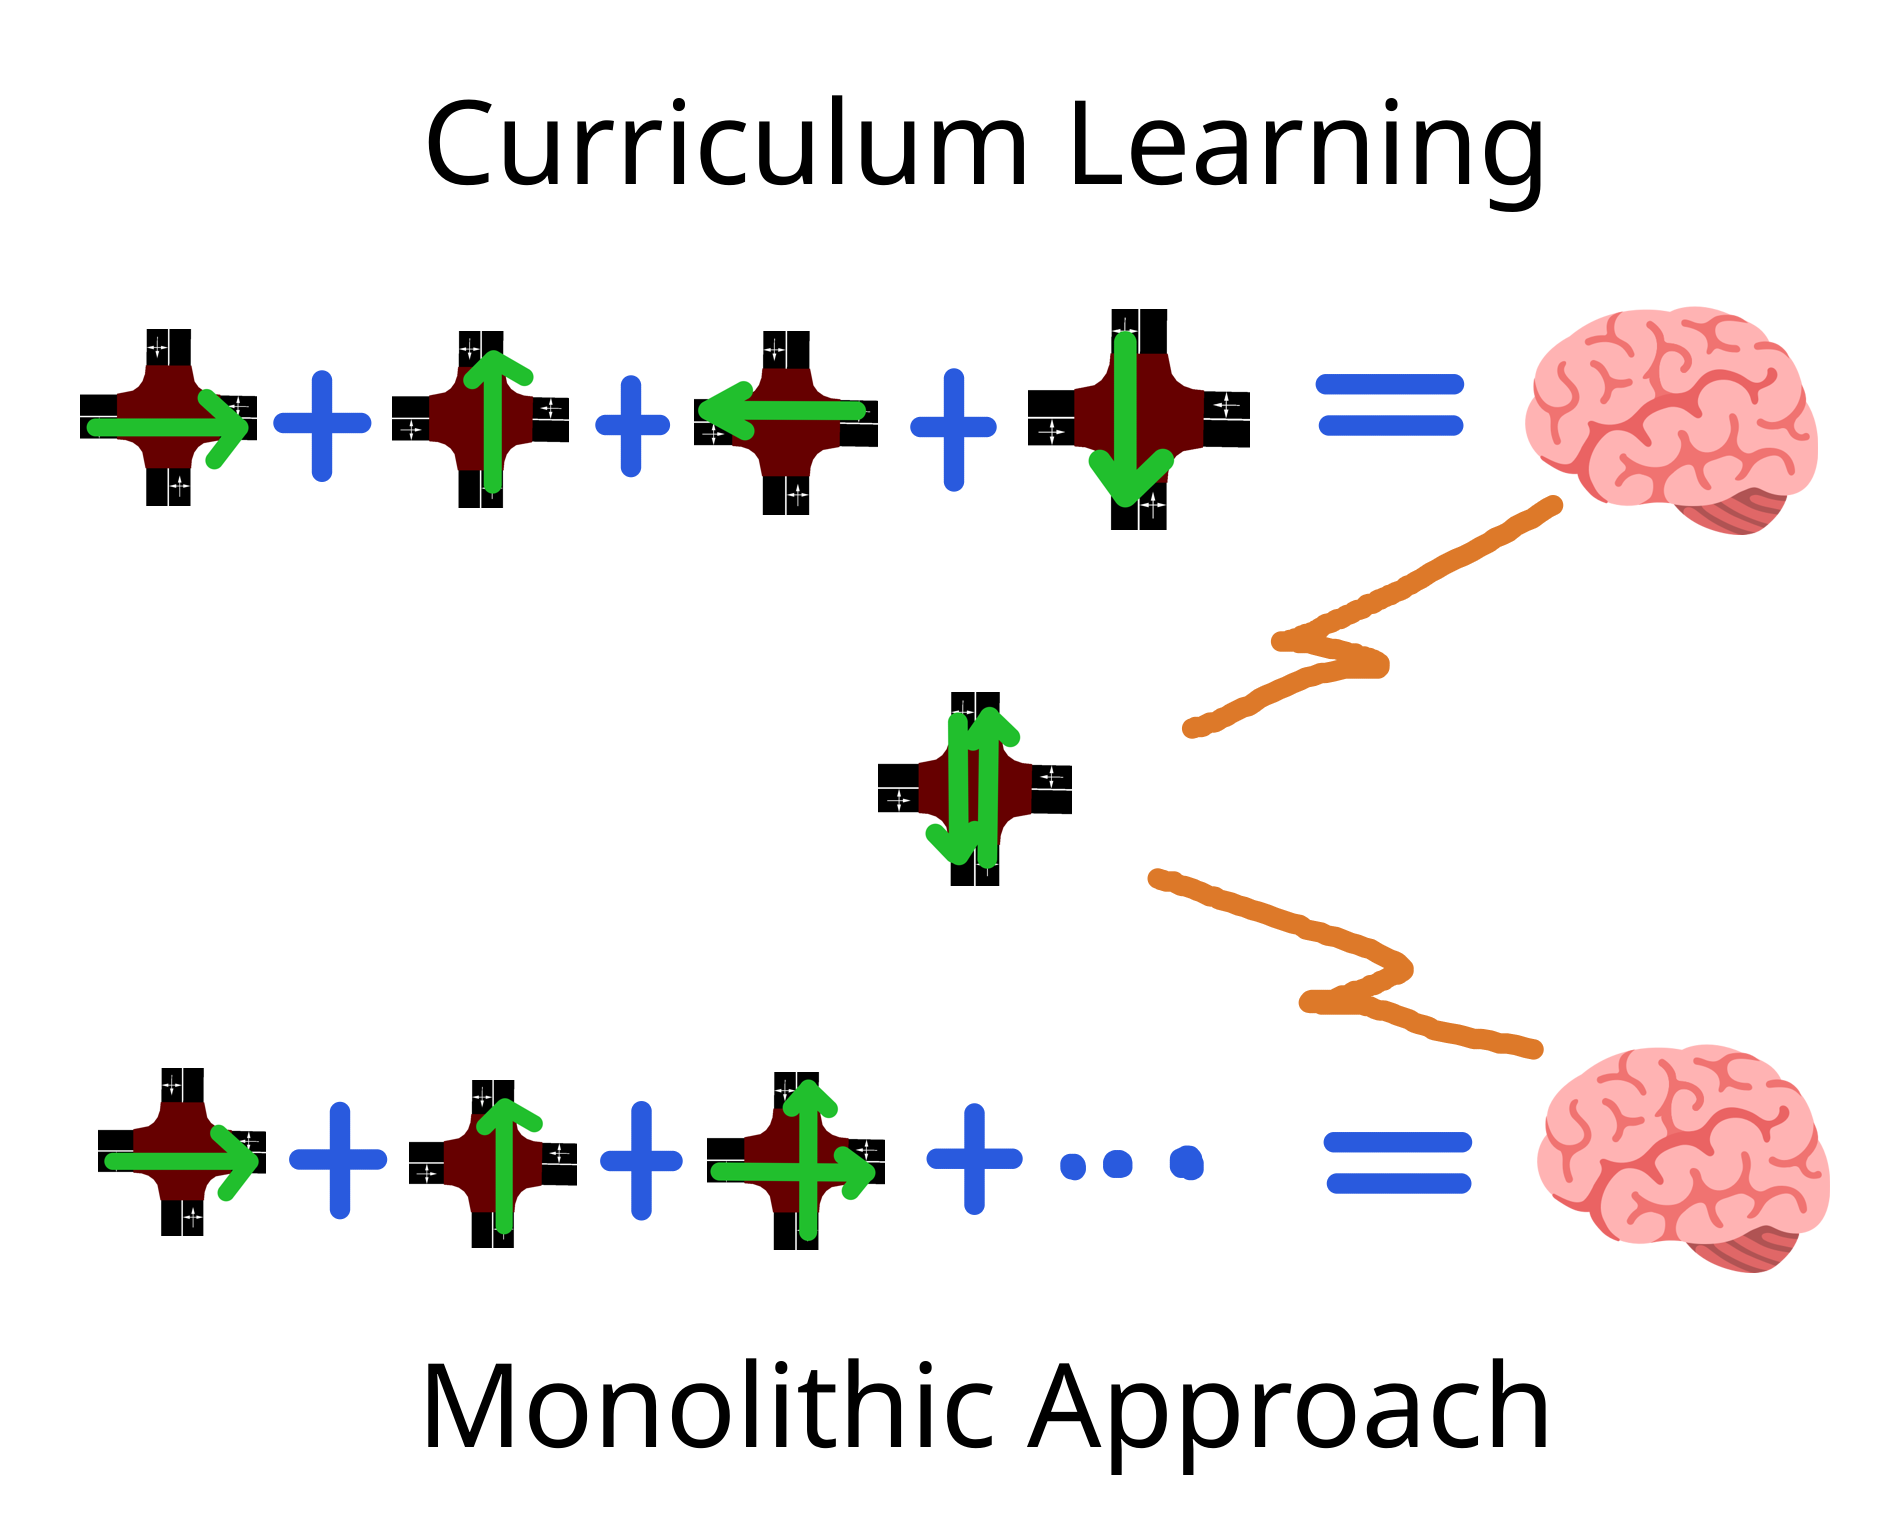
\includegraphics[width=0.75\textwidth]{figures/curriculum-vs-monolithic.png}
  \end{figure}
\end{frame}

\begin{frame}
\frametitle{Experimental results}
  \begin{columns}
  \begin{column}{0.5\textwidth}
    \begin{figure}
      \centering
      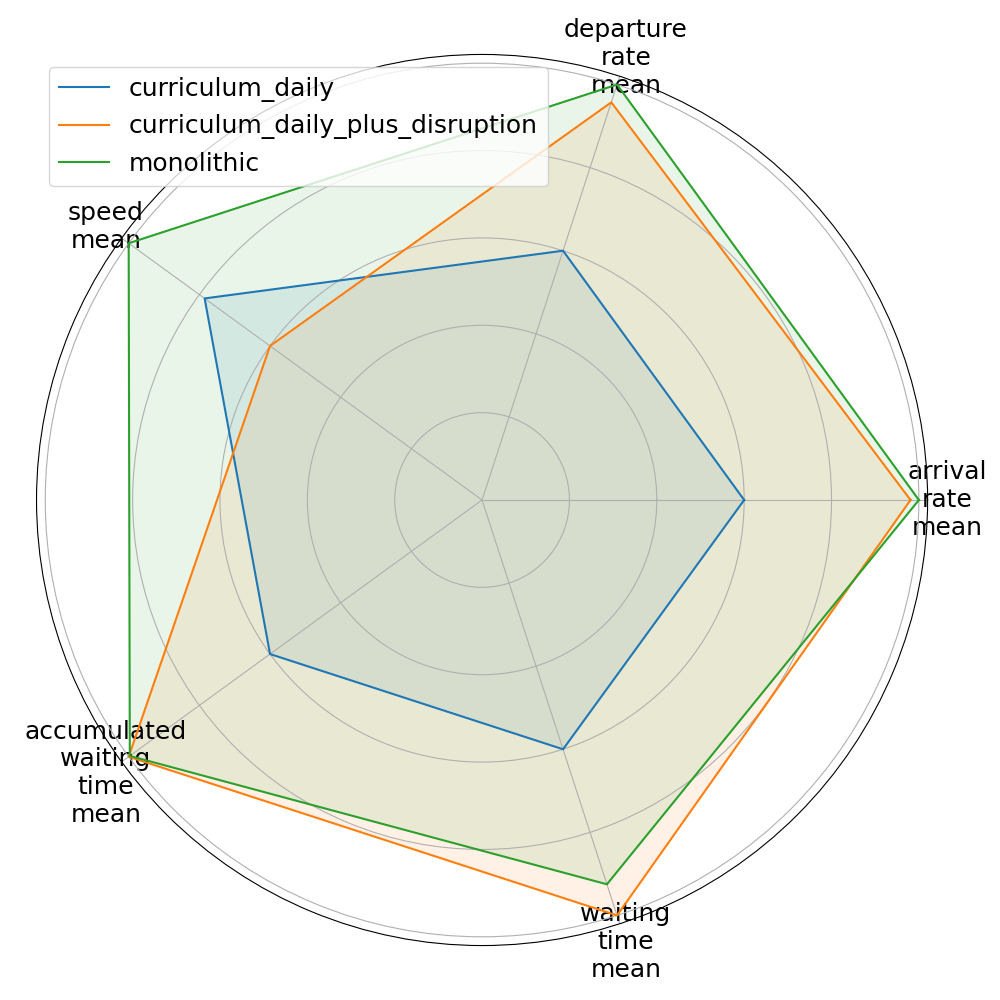
\includegraphics[width=1.0\textwidth]{figures/dataset-radar.png}
    \end{figure}
  \end{column}
  \begin{column}{0.5\textwidth}
    \begin{itemize}
      \item TODO
    \end{itemize}
  \end{column}
\end{columns}
\end{frame}

\begin{frame}
  \begin{figure}
    \centering
    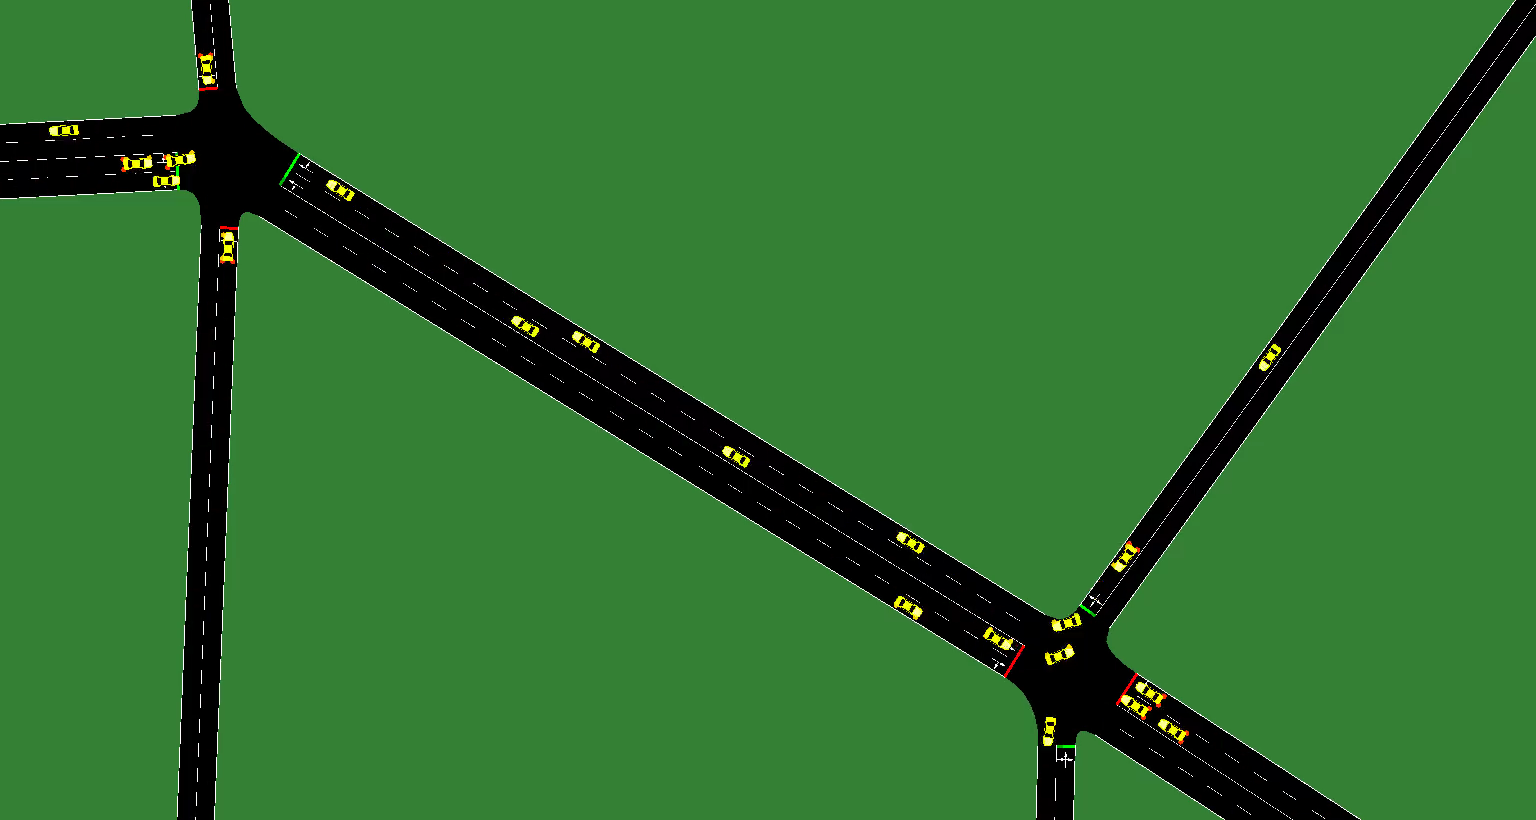
\includegraphics[width=0.5\textwidth]{figures/demo.clr.mon.png}
    \caption{Monolithic}
  \end{figure}
  \begin{columns}
    \begin{column}{0.5\textwidth}
      \begin{figure}
        \centering
        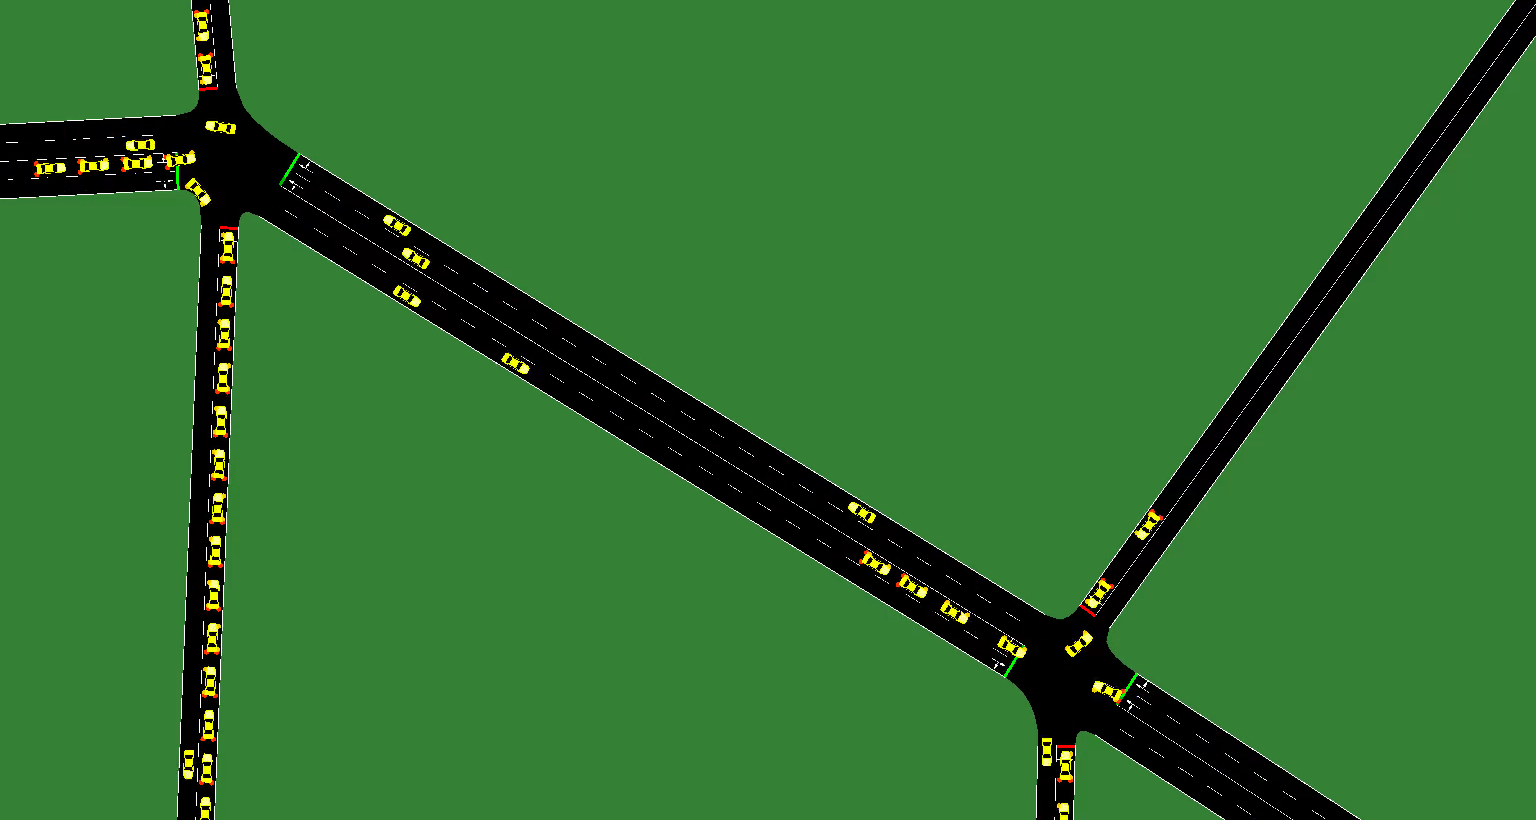
\includegraphics[width=1.0\textwidth]{figures/demo.clr.cd.png}
        \caption{Curriculum Daily}
      \end{figure}
    \end{column}
    \begin{column}{0.5\textwidth}
      \begin{figure}
        \centering
        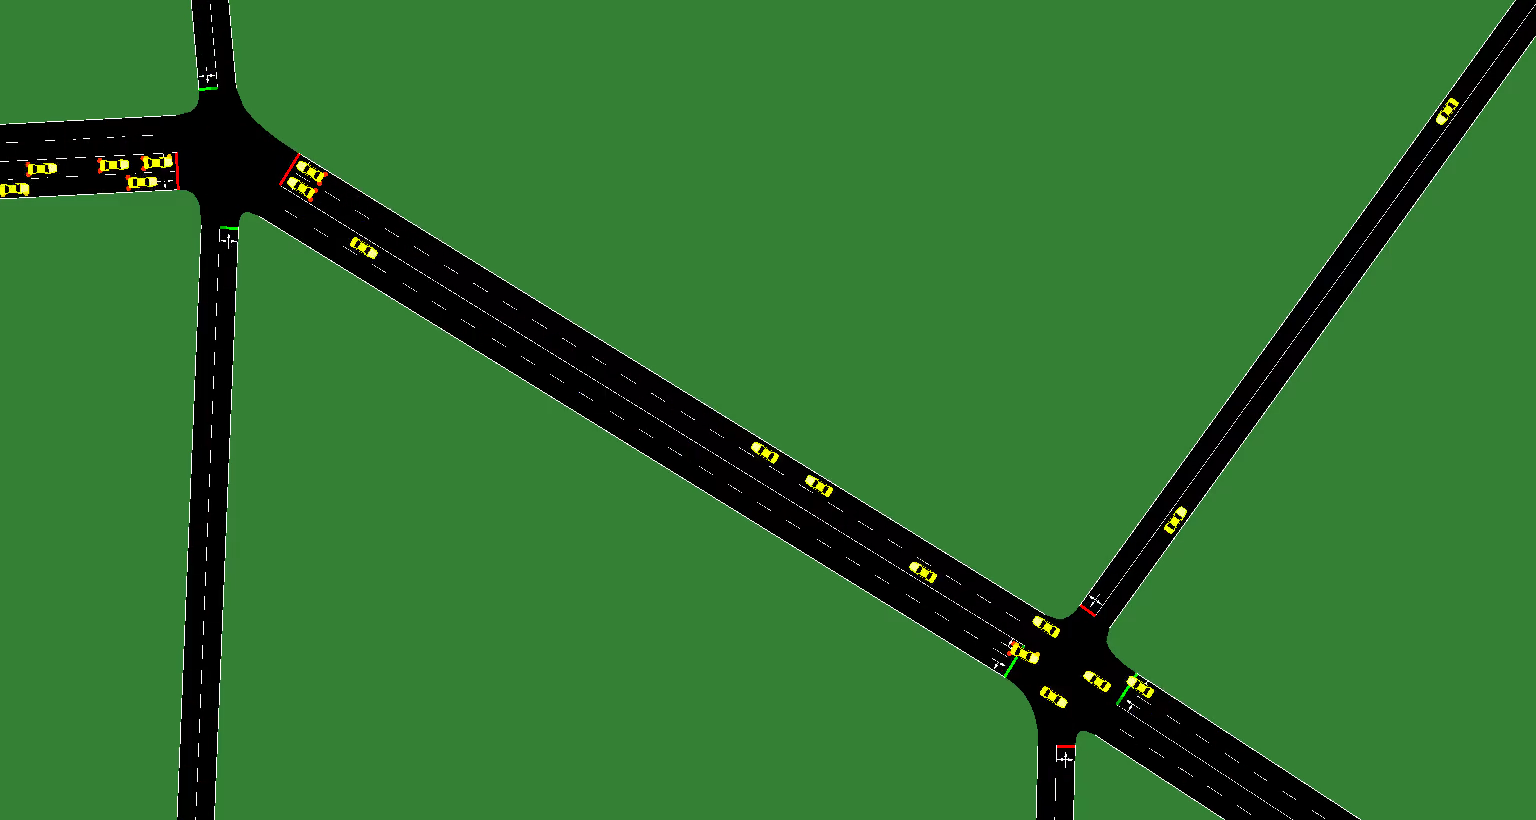
\includegraphics[width=1.0\textwidth]{figures/demo.clr.cdd.png}
        \caption{Curriculum Daily + Disruption}
      \end{figure}
    \end{column}
  \end{columns}
\end{frame}

\section{Multi Agent Learning}
\begin{frame}
\centering
\Huge
Multi Agent Learning
\end{frame}

\begin{frame}
\frametitle{Multi Agent Learning}

  {\footnotesize
  \begin{itemize}
    \item No agent is isoled, they are all part of a whole and they influence each other with their own behaviour.
    \item What if an agent can \textit{sense} its surrounding area by sharing observations with neighbours?
    \item What if an agent is \textit{rewarded} for its influence on surrounding area by sharing rewards with neighbours?
  \end{itemize}
  }

  \begin{columns}
    \begin{column}{0.3\textwidth}
      \begin{figure}
        \centering
        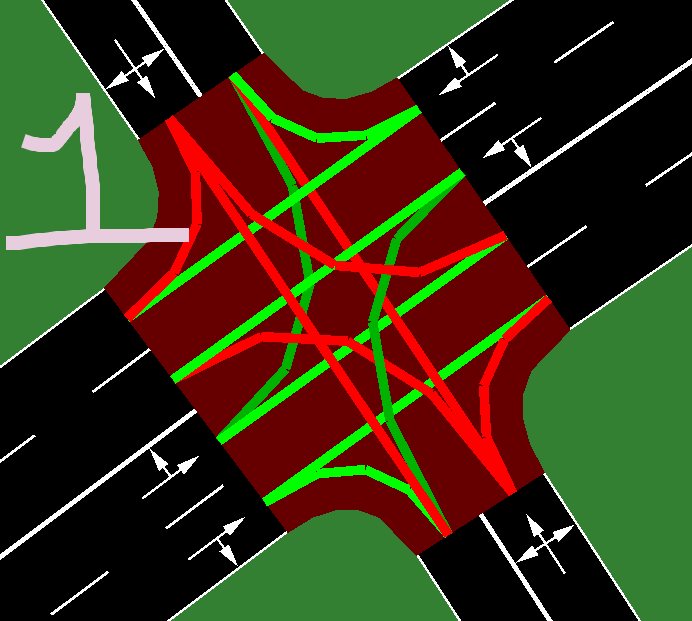
\includegraphics[width=0.65\textwidth]{figures/sumo-rf-tls-1.png}
      \end{figure}
    \end{column}
    \begin{column}{0.3\textwidth}
      \begin{figure}
        \centering
        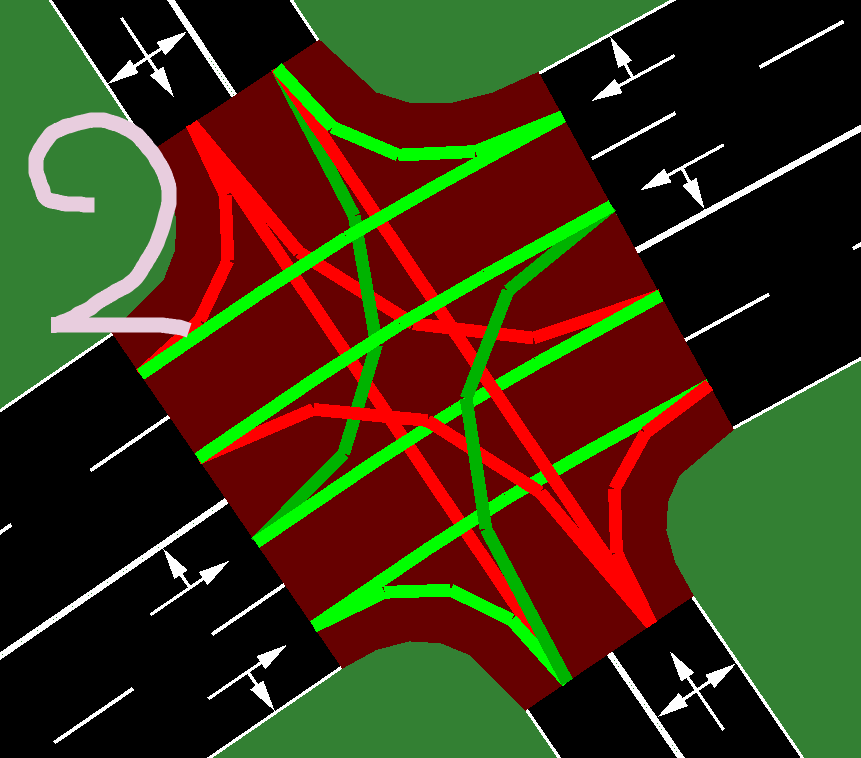
\includegraphics[width=0.65\textwidth]{figures/sumo-rf-tls-2.png}
      \end{figure}
    \end{column}
    \begin{column}{0.3\textwidth}
      \begin{figure}
        \centering
        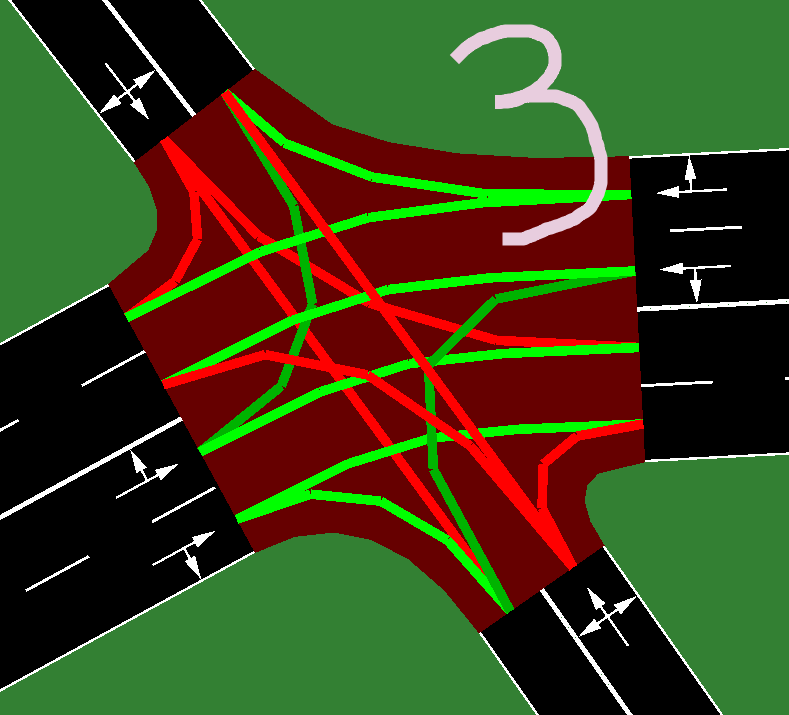
\includegraphics[width=0.65\textwidth]{figures/sumo-rf-tls-3.png}
      \end{figure}
    \end{column}
  \end{columns}
  \begin{columns}
    \begin{column}{0.5\textwidth}
      \begin{figure}
        \centering
        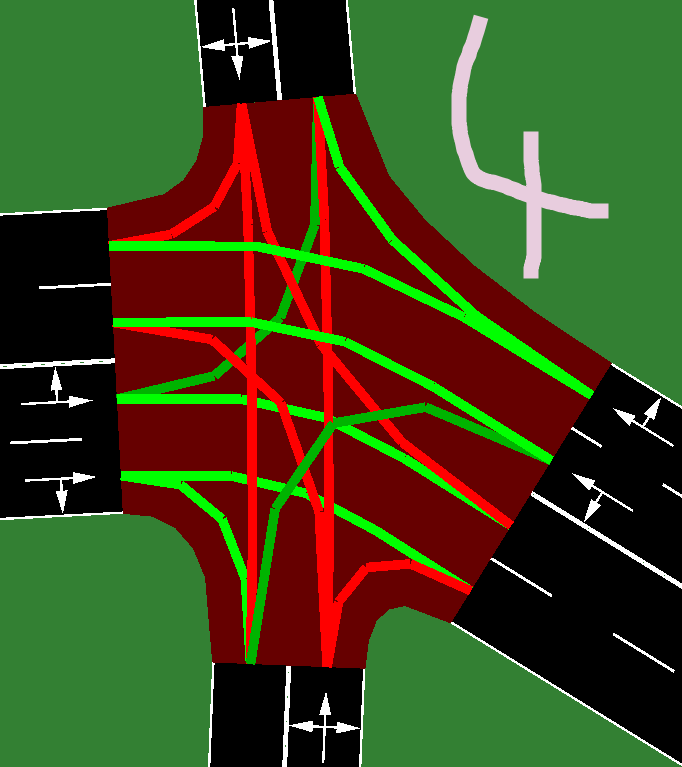
\includegraphics[width=0.30\textwidth]{figures/sumo-rf-tls-4.png}
      \end{figure}
    \end{column}
    \begin{column}{0.5\textwidth}
      \begin{figure}
        \centering
        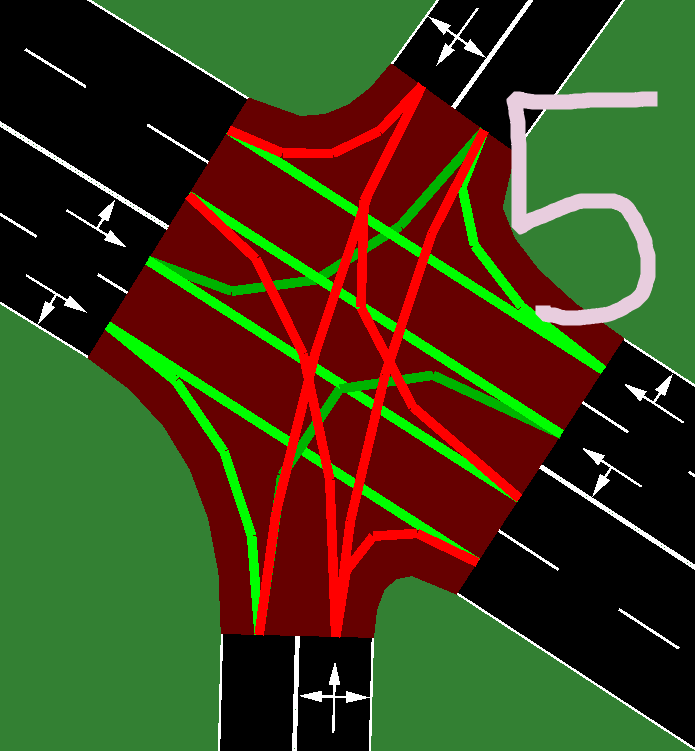
\includegraphics[width=0.30\textwidth]{figures/sumo-rf-tls-5.png}
      \end{figure}
    \end{column}
  \end{columns}
\end{frame}

\begin{frame}
\frametitle{Observation sharing}

  {\footnotesize
  \begin{itemize}
    \item The state $S$ of an agent is computed through two dinstict observation functions $f_{int}, f_{ext}$ meaning respectively the internal state and external state. \\
    \item The state of an agent $x$ is a concatenation of $f_{int}(x)$ and $f_{ext}(y)$ for all $y \in N(x)$, where $N$ is a function mapping an agent with its neighbours. \\
    \item It ws chosen to use the Density function as $f_{int}$ because, among the observation functions where the agent can only see itself, it produced the best results.
  \end{itemize}
  }

  Example:
  \begin{figure}
    \centering
    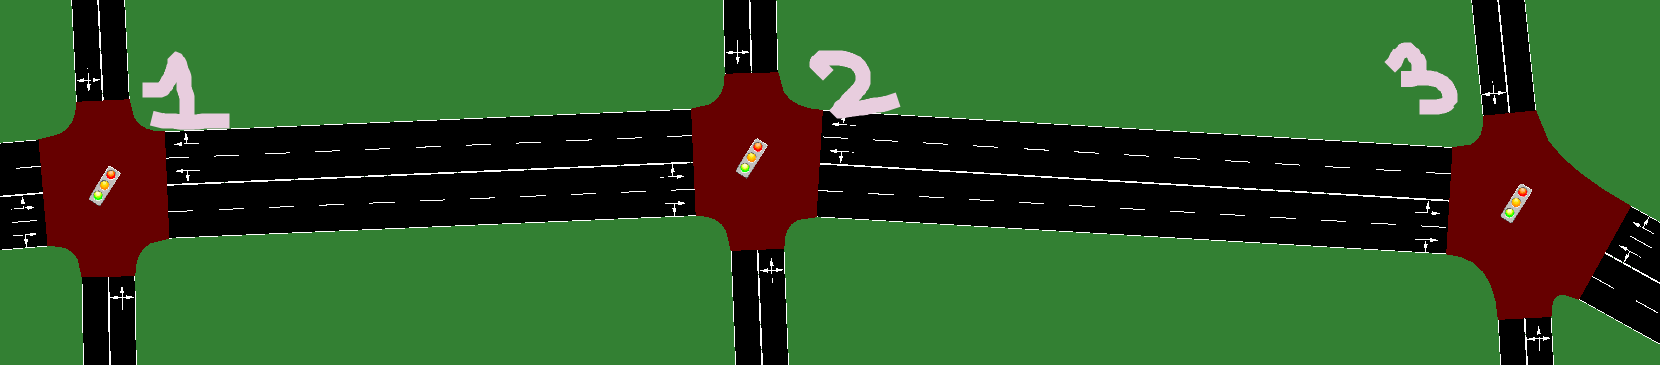
\includegraphics[width=0.75\textwidth]{figures/sumo-rf-tls-triplet.png}
  \end{figure}

  
  \begin{columns}
    \begin{column}{0.4\textwidth}
      \centering
      {\footnotesize$S({TLS}_{1}) = f_{int}({TLS}_{1}) \bullet f_{ext}({TLS}_{2})$}
    \end{column}
    \begin{column}{0.6\textwidth}
      \centering
      {\footnotesize$S({TLS}_{2}) = f_{int}({TLS}_{2}) \bullet f_{ext}({TLS}_{1}) \bullet f_{ext}({TLS}_{3})$}
    \end{column}
  \end{columns}
\end{frame}

\begin{frame}
\frametitle{Experimental results}
  \begin{columns}
  \begin{column}{0.5\textwidth}
    \begin{figure}
      \centering
      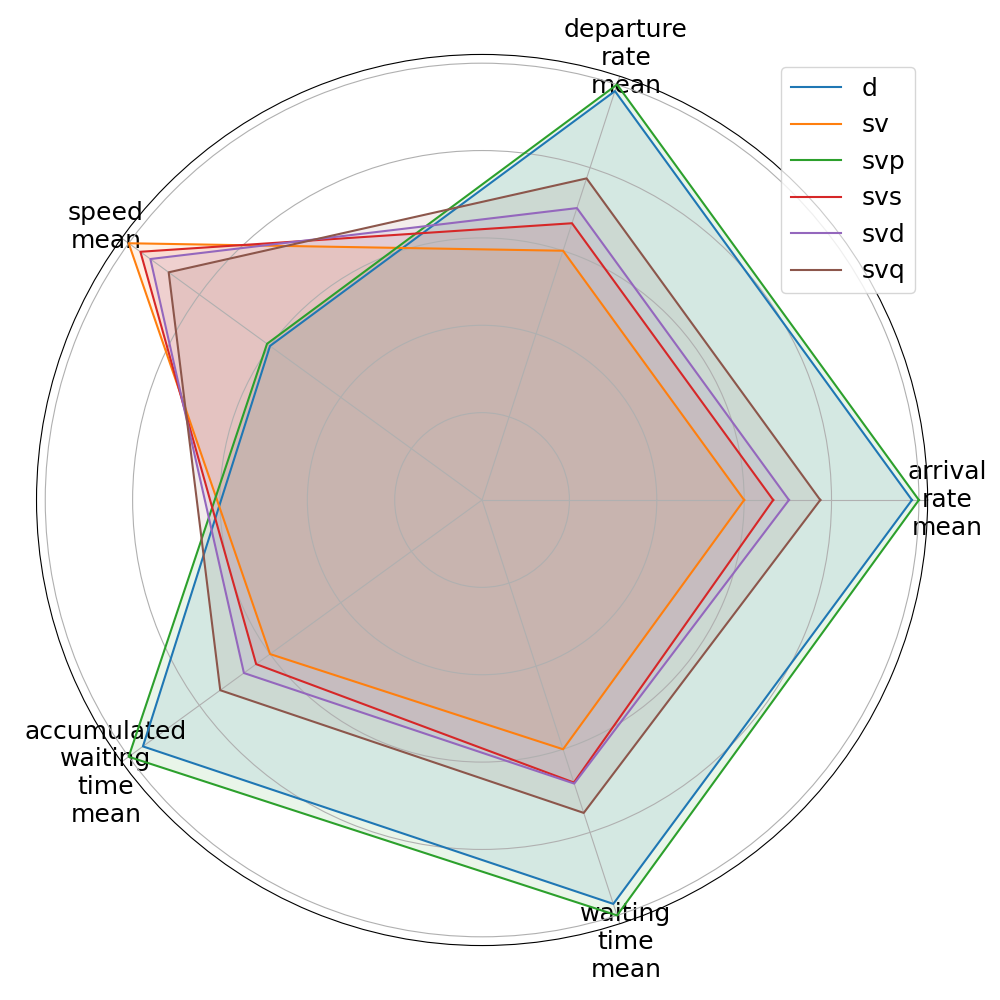
\includegraphics[width=1.0\textwidth]{figures/obs-sharing-radar.png}
    \end{figure}
  \end{column}
  \begin{column}{0.5\textwidth}
    \begin{itemize}
      \item TODO
    \end{itemize}
  \end{column}
\end{columns}
\end{frame}

\begin{frame}
\frametitle{Reward sharing}

  {\footnotesize
  \begin{itemize}
    \item The reward $R$ of an agent is computed through one single reward function $f$ representing the condition of an intersection. \\
    \item The state of an agent $x$ is a sum of $f(x)$ and $f(y)$ for all $y \in N(x)$, where $N$ is a function mapping an agent with its neighbours. \\
  \end{itemize}
  }

  Example:
  \begin{figure}
    \centering
    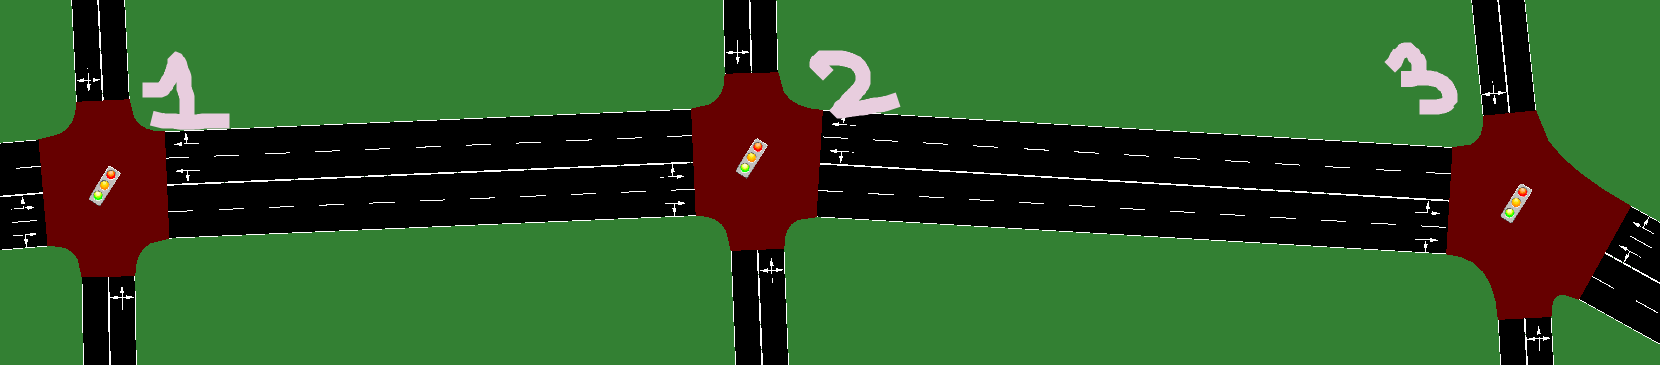
\includegraphics[width=0.75\textwidth]{figures/sumo-rf-tls-triplet.png}
  \end{figure}

  
  \begin{columns}
    \begin{column}{0.4\textwidth}
      \centering
      {\footnotesize$R({TLS}_{1}) = f({TLS}_{1}) + f({TLS}_{2})$}
    \end{column}
    \begin{column}{0.6\textwidth}
      \centering
      {\footnotesize$R({TLS}_{2}) = f({TLS}_{2}) + f({TLS}_{1}) + f({TLS}_{3})$}
    \end{column}
  \end{columns}
\end{frame}

\begin{frame}
\frametitle{Experimental results}
  \begin{columns}
  \begin{column}{0.5\textwidth}
    \begin{figure}
      \centering
      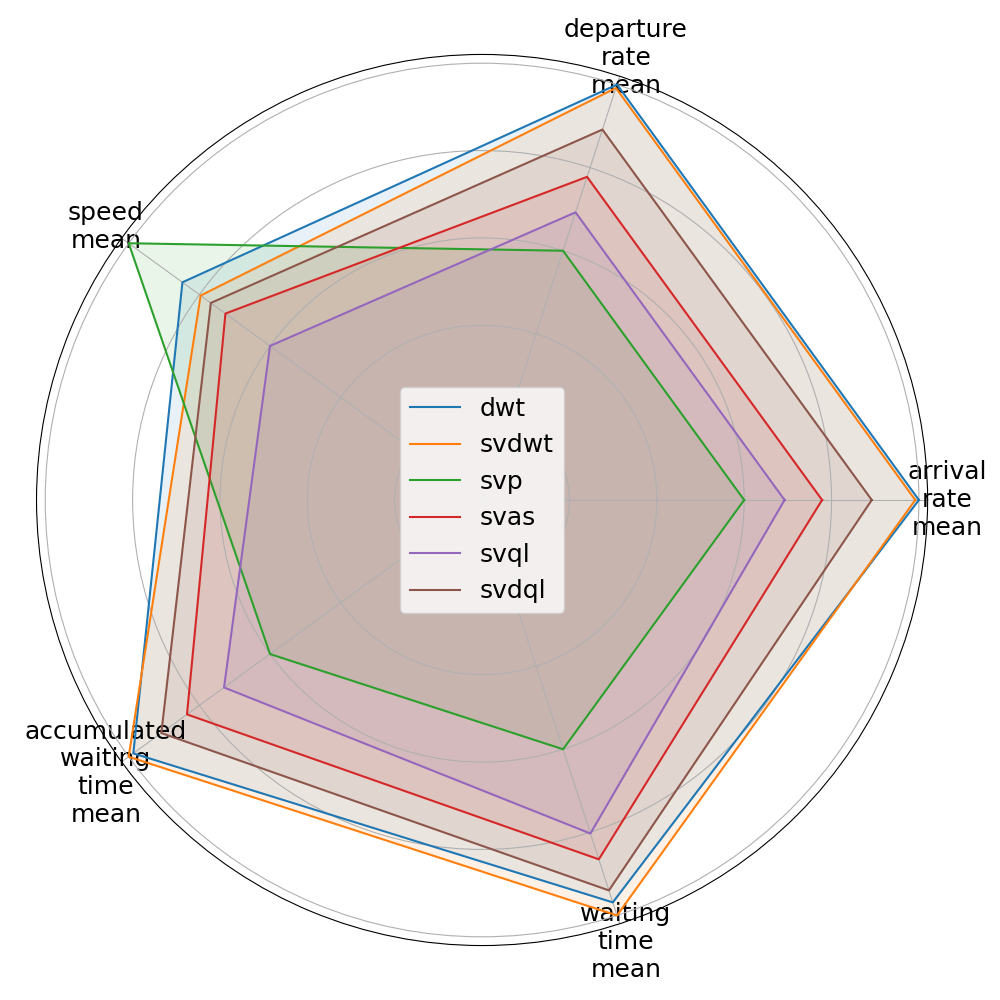
\includegraphics[width=1.0\textwidth]{figures/rew-sharing-radar.png}
    \end{figure}
  \end{column}
  \begin{column}{0.5\textwidth}
    \begin{itemize}
      \item TODO
    \end{itemize}
  \end{column}
\end{columns}
\end{frame}

\begin{frame}
  \begin{itemize}
    \item With sharing emerges a green-wave phenomenon
  \end{itemize}

  \begin{columns}
    \begin{column}{0.5\textwidth}
      \begin{figure}
        \centering
        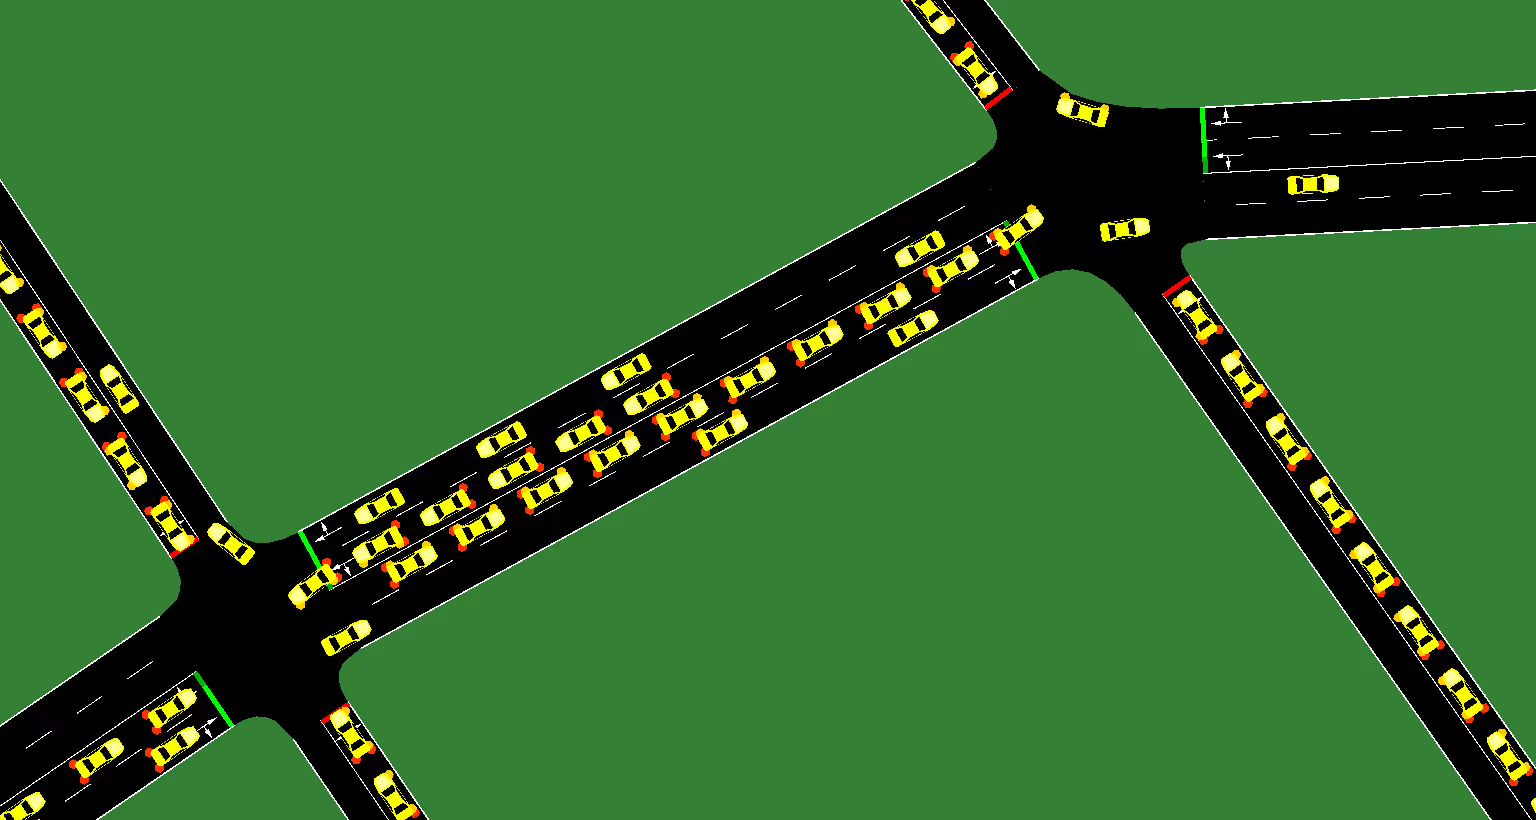
\includegraphics[width=0.85\textwidth]{figures/dql-shared.0.png}
      \end{figure}
    \end{column}
    \begin{column}{0.5\textwidth}
      \begin{figure}
        \centering
        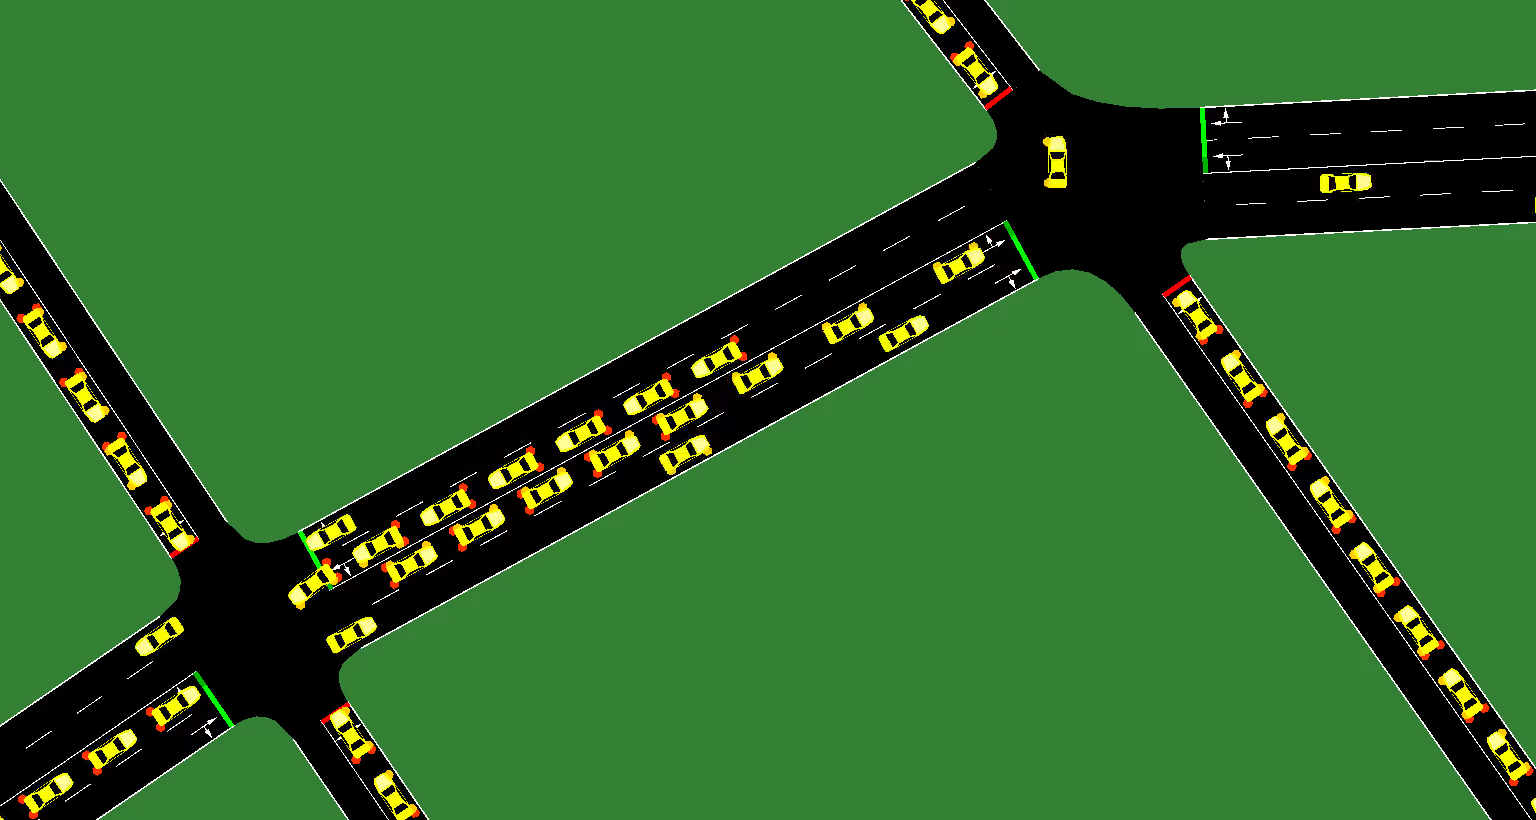
\includegraphics[width=0.85\textwidth]{figures/dql-shared.1.png}
      \end{figure}
    \end{column}
  \end{columns}

  \vspace{3mm}
  \begin{itemize}
    \item Without sharing flows are more segmented
  \end{itemize}
  
  \begin{columns}
    \begin{column}{0.5\textwidth}
      \begin{figure}
        \centering
        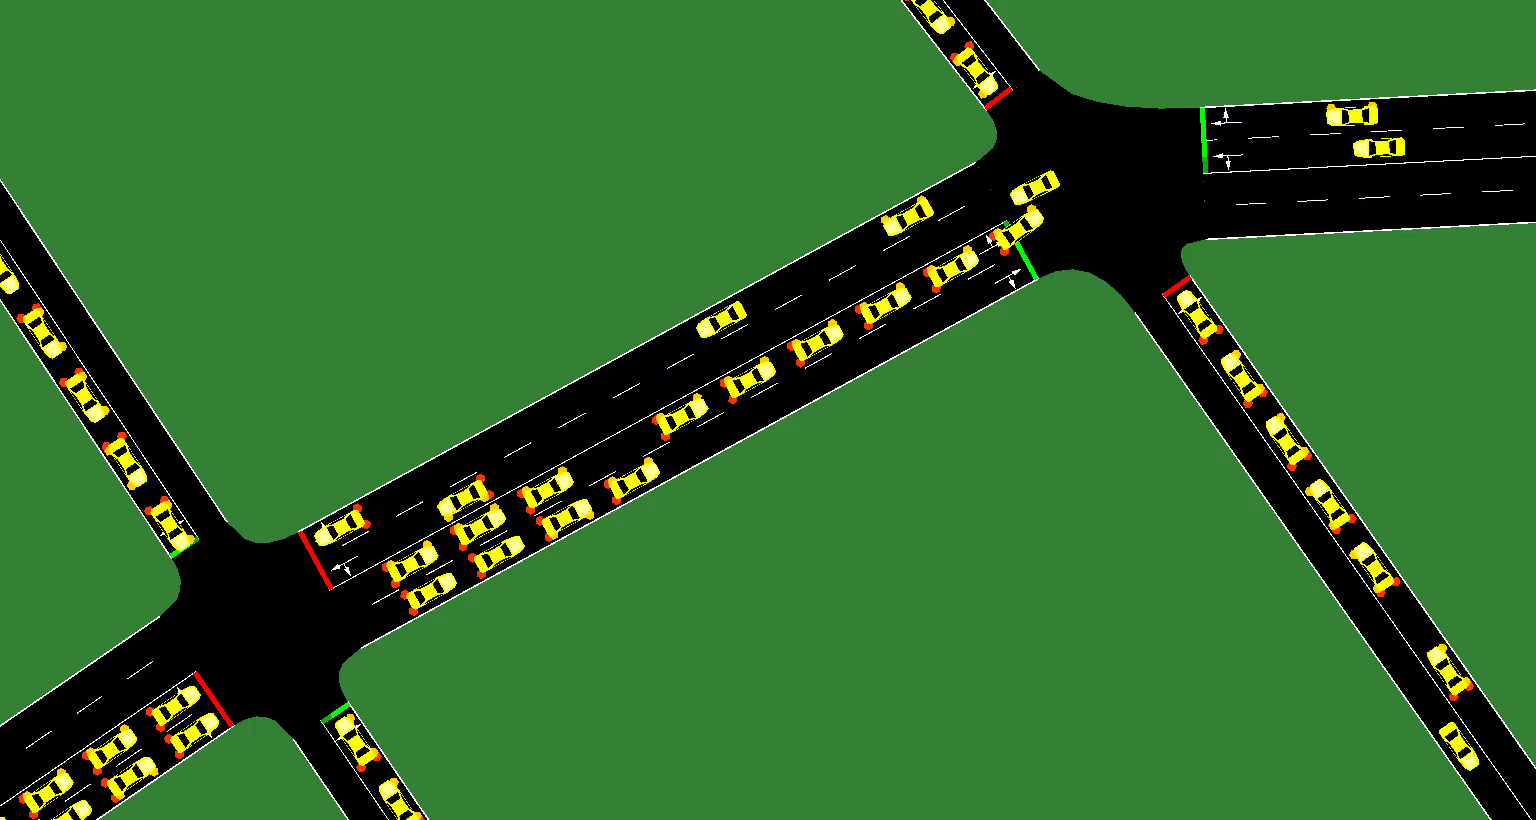
\includegraphics[width=0.85\textwidth]{figures/dql-unshared.0.png}
      \end{figure}
    \end{column}
    \begin{column}{0.5\textwidth}
      \begin{figure}
        \centering
        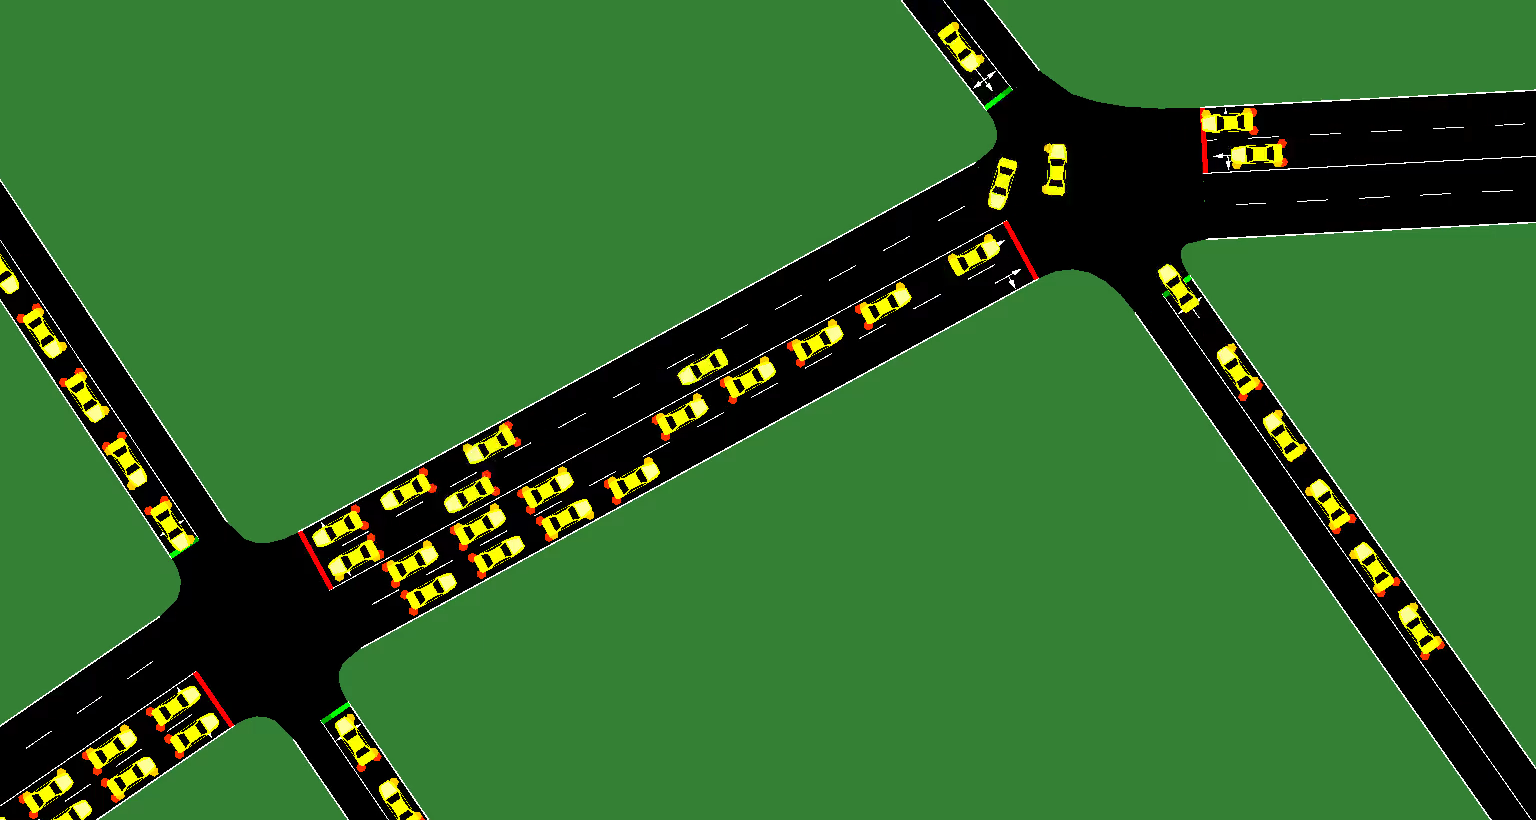
\includegraphics[width=0.85\textwidth]{figures/dql-unshared.1.png}
      \end{figure}
    \end{column}
  \end{columns}
\end{frame}

%[fragile]
% \begin{small}
%   \begin{verbatim}
%   TOK = (£|\*|~|%(,[0-9.]+)?(,[0-9.]+)?|[A-Z][A-Z0-9]+)
%   EXP = ^([0-9]+,)?([0-9]+,)?TOK(,TOK)*$
%   \end{verbatim}
% \end{small}

\section{Conclusions}
\begin{frame}
\centering
\Huge
Conclusions
\end{frame}

\begin{frame}
  \frametitle{Take-away}
  Conclusions:
  \begin{itemize}
    \item Curriculum based approaches are simple and cheap but as effective as exhaustive approaches
    \item RL-based traffic light control benefits from Multi Agent Learning
  \end{itemize}

  Future work:
  \begin{itemize}
    \item Experiment with wider networks and longer training times
    \item Apply transfer learning to heterogeneous agents
    \item Experiment with Experience Replay
  \end{itemize}
\end{frame}

\begin{frame}
\centering
\Huge
Bonus
\end{frame}

\begin{frame}
\frametitle{A matter of perspective}
  \begin{columns}
  \begin{column}{0.5\textwidth}
    \begin{figure}
      \centering
      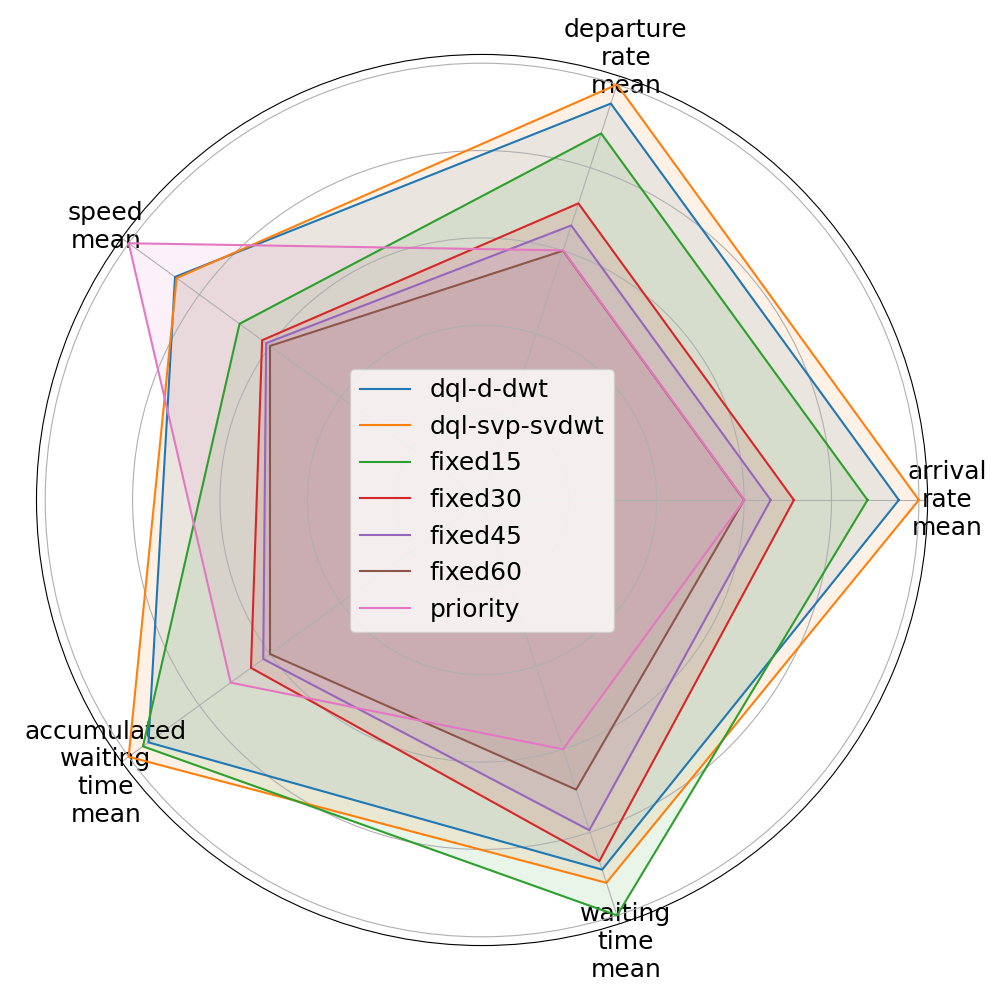
\includegraphics[width=1.0\textwidth]{figures/total-radar.png}
    \end{figure}
  \end{column}
  \begin{column}{0.5\textwidth}
    \begin{itemize}
      \item TODO
    \end{itemize}
  \end{column}
\end{columns}
\end{frame}

\begin{frame}
  \begin{columns}
    \begin{column}{0.5\textwidth}
      \begin{figure}
        \centering
        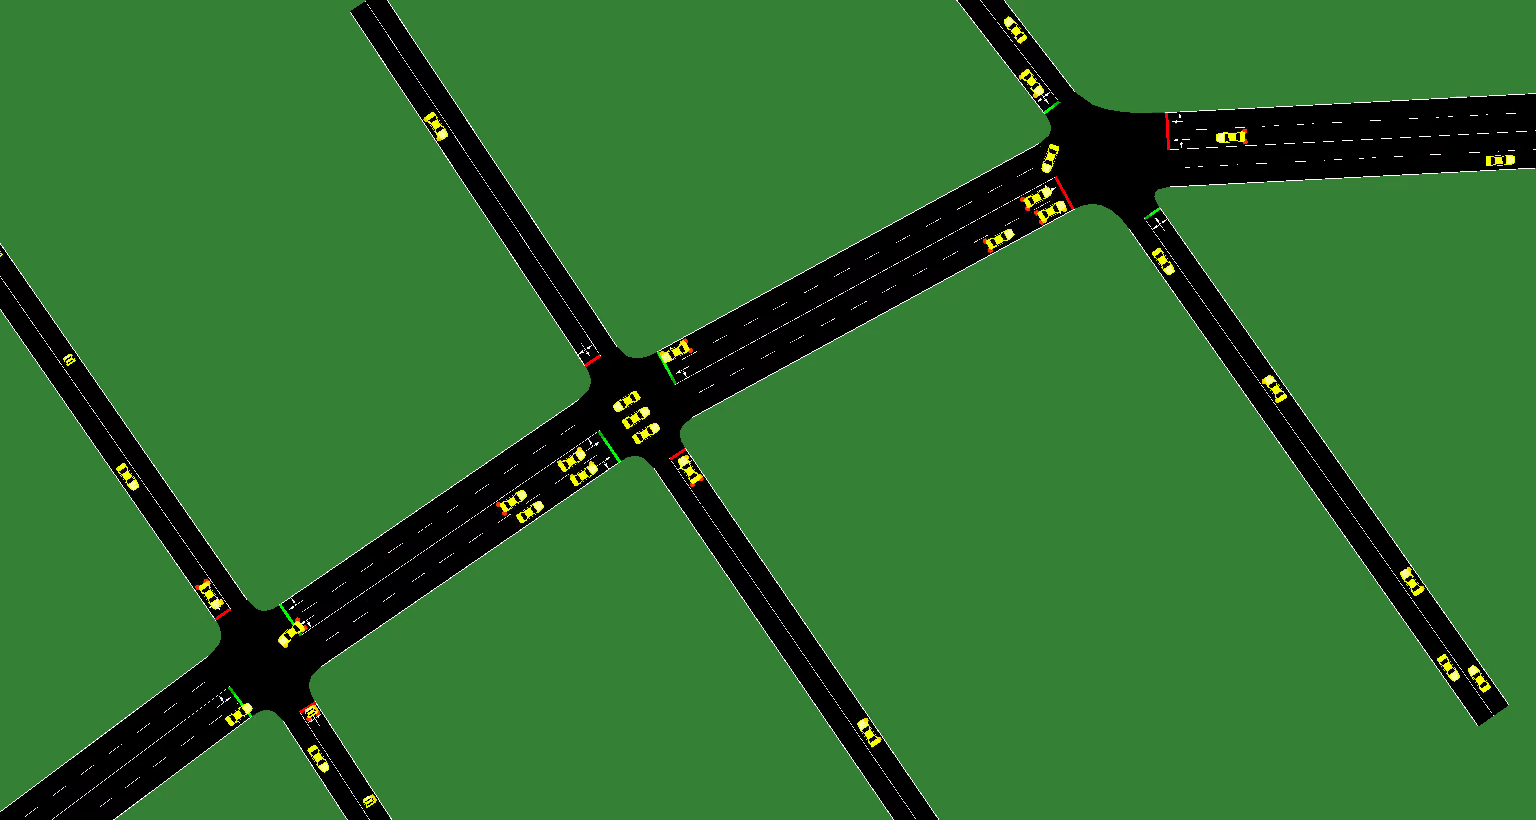
\includegraphics[width=1.0\textwidth]{figures/demo.dql-d-dwt.png}
        \caption{DQL Agent}
      \end{figure}
    \end{column}
    \begin{column}{0.5\textwidth}
      \begin{figure}
        \centering
        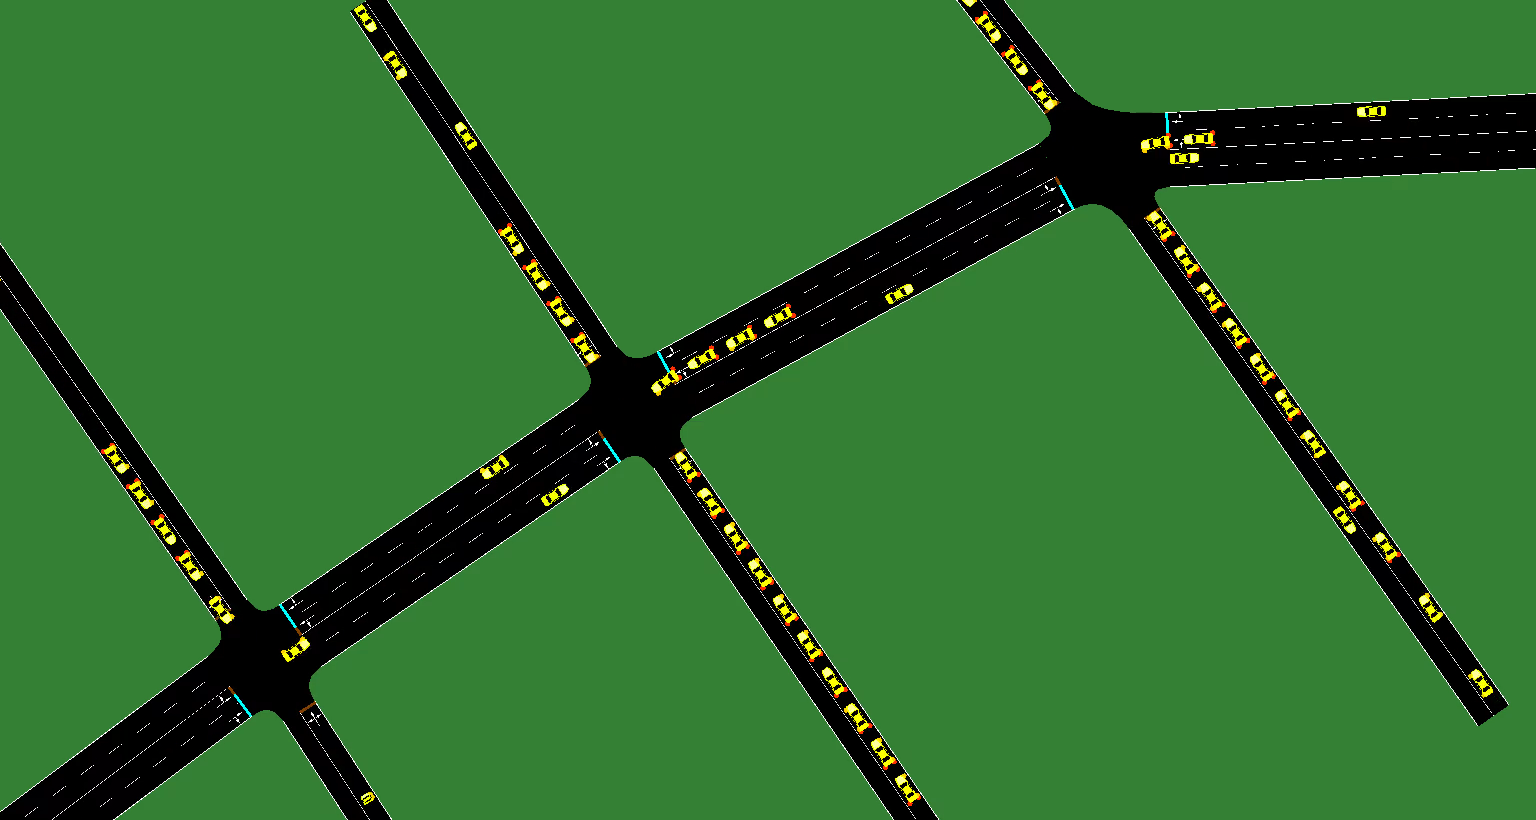
\includegraphics[width=1.0\textwidth]{figures/demo.priority.png}
        \caption{Unregulated}
      \end{figure}
    \end{column}
  \end{columns}
  \begin{columns}
    \begin{column}{0.5\textwidth}
      \begin{figure}
        \centering
        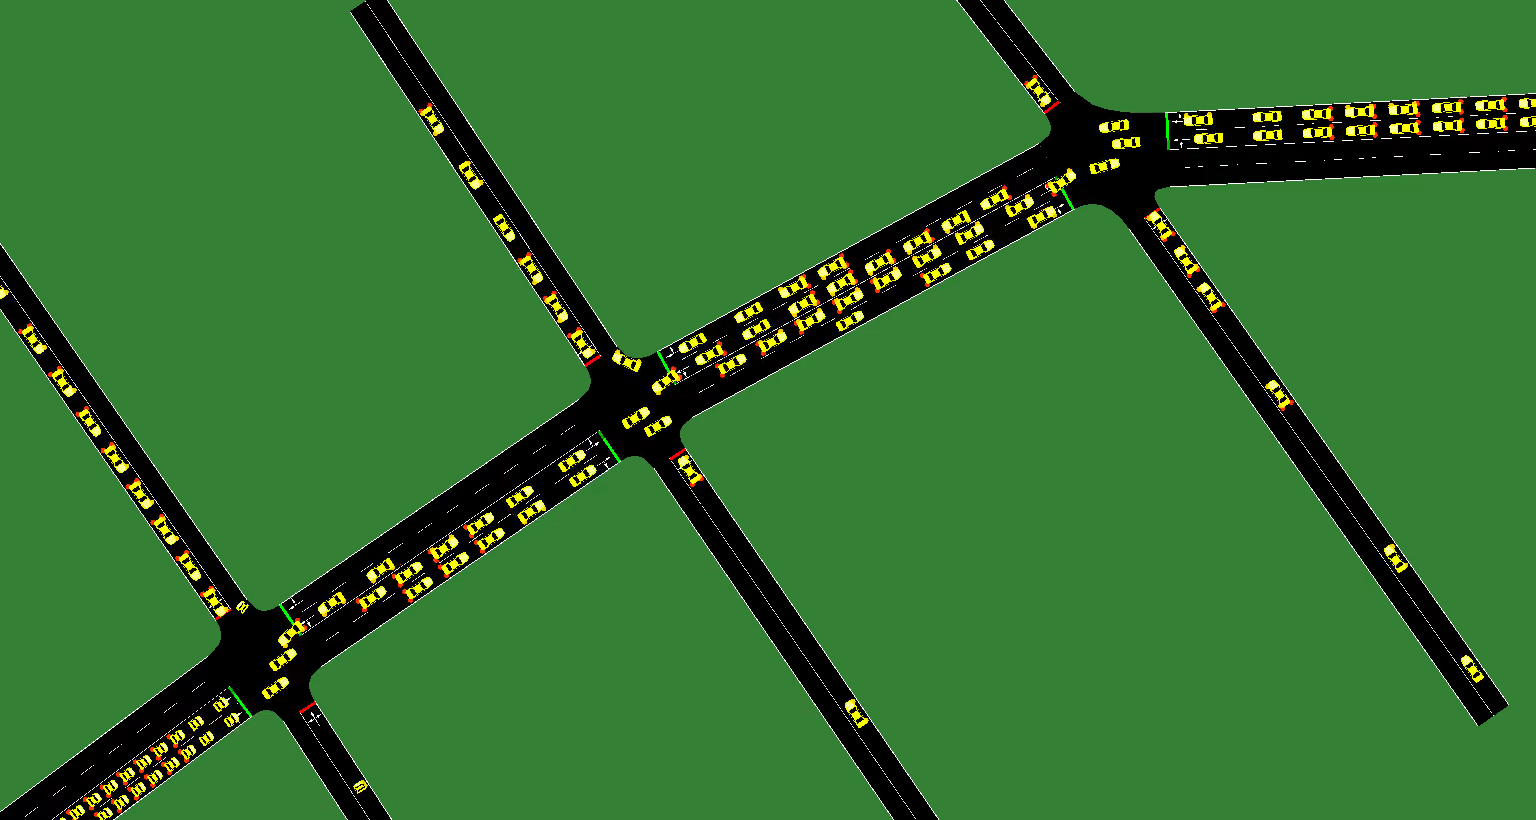
\includegraphics[width=1.00\textwidth]{figures/demo.fixed15.png}
        \caption{Fixed Cycle 15s}
      \end{figure}
    \end{column}
    \begin{column}{0.5\textwidth}
      \begin{figure}
        \centering
        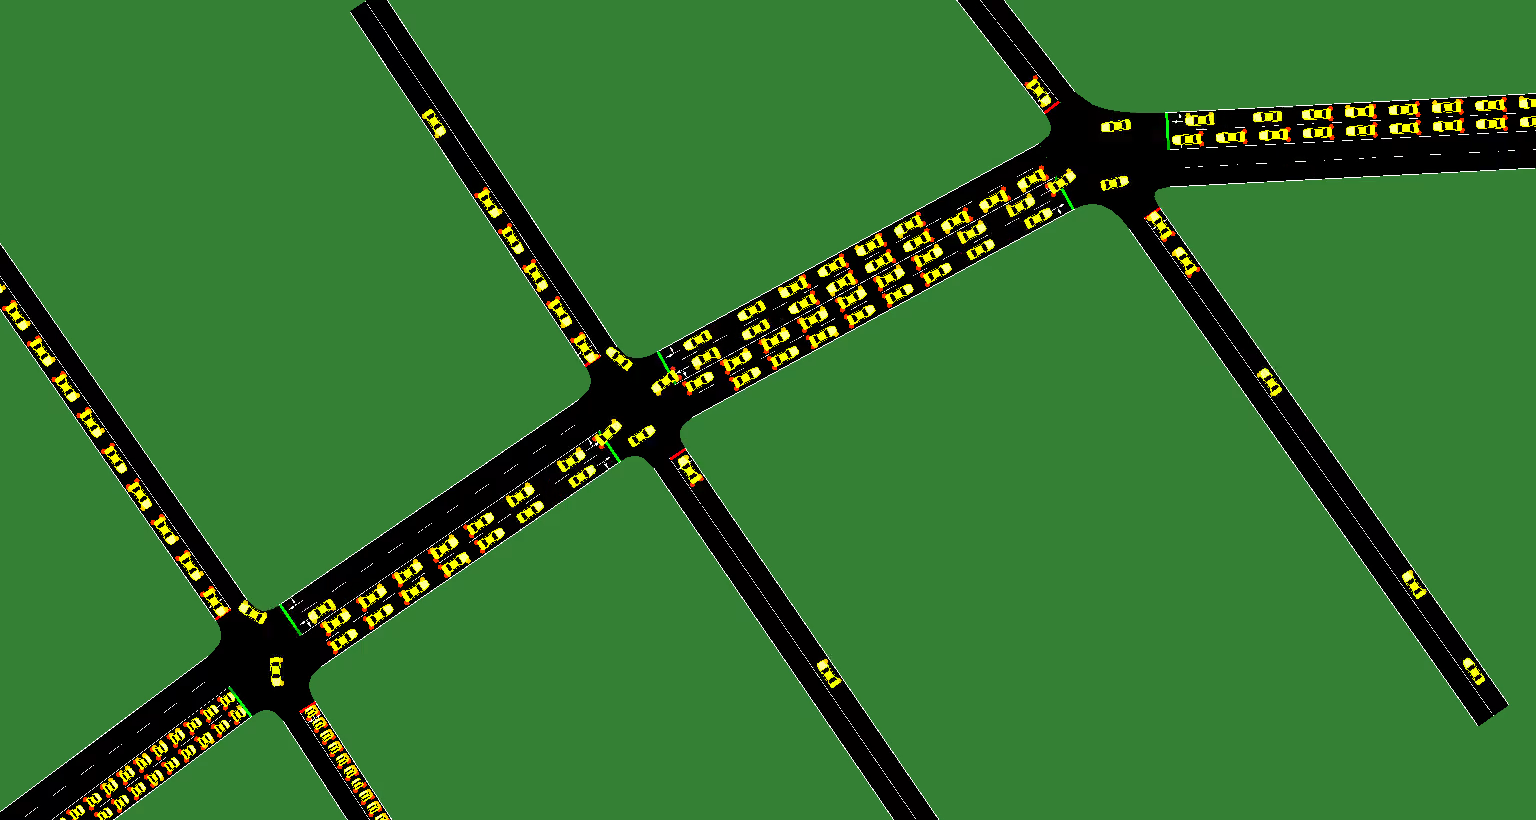
\includegraphics[width=1.00\textwidth]{figures/demo.fixed60.png}
        \caption{Fixed Cycle 60s}
      \end{figure}
    \end{column}
  \end{columns}
\end{frame}

\begin{frame}
\centering
\Huge
Thank You
\end{frame}

\end{document}
